\documentclass[12pt]{article}
\usepackage{anyfontsize}
\usepackage[a4paper, margin=2cm]{geometry}
\usepackage{polski}
\usepackage{tabto}
\usepackage{enumitem}
\usepackage{amsmath}
\usepackage{amssymb}
\usepackage{multirow}
\usepackage{multicol}
\usepackage{setspace}
\usepackage{listings}
\usepackage{titlesec}
\titlelabel{\thetitle.\quad}
% \AddToHook{cmd/section/before}{\clearpage}
\usepackage[title,toc,page]{appendix}
\usepackage{lipsum}
\usepackage{pdflscape}
\makeatletter
\newcommand{\newgeometryfull}[1]{%
  \clearpage
  \Gm@restore@org
  \Gm@initnewgm
 % \Gm@newgmtrue
  \setkeys{Gm}{#1}%
%  \Gm@newgmfalse
  \Gm@process
  \ifnum\mag=\@m\else\Gm@magtooffset\fi
  \Gm@changelayout
  \Gm@showparams{newgeometry}}%
\makeatother


\newcommand*\useBigLandscape{%
    \newgeometryfull{a3paper,landscape, width=360mm, top = 20mm, bottom = 25mm}
    % \newgeometry{a3paper, landscape}
    % set the correct dimension for the PDF viewer
    \pdfpageheight=297mm
    \pdfpagewidth=420mm
}

\newcommand*\useNormalLandscape{%
    \newgeometryfull{a4paper,landscape, width=257mm, top = 15mm, bottom = 15mm}
    % set the correct dimension for the PDF viewer
    \pdfpageheight=210mm
    \pdfpagewidth=297mm
}

\newcommand*\useportrait{%
    \restoregeometry
    \clearpage
    % set the correct dimension for the PDF viewer
    \pdfpageheight=297mm
    \pdfpagewidth=210mm
}

\setlength{\emergencystretch}{10pt}


\usepackage{tabularx}
\newcolumntype{C}{>{\centering\arraybackslash}X}
\newcolumntype{L}{>{\raggedleft\arraybackslash}X}
\newcolumntype{R}{>{\raggedright\arraybackslash}X}
\newcommand{\centerY}[2]{\multirow{#1}{*}{#2}}

\usepackage{wrapfig}

\usepackage{chngcntr}
\counterwithin{figure}{section}
\counterwithin{table}{section}
\numberwithin{equation}{section}

\usepackage{hyperref}
\hypersetup{
    colorlinks = true,
    urlcolor=blue,
    linkcolor= black,
    citecolor= blue
}

\usepackage{graphicx}
\graphicspath{{./Img/}}

\usepackage{csvsimple}
\usepackage{pgfplots}
\usepackage{pgfplotstable}
\pgfplotsset{compat= newest}


\usepackage{titlesec}
\titlelabel{\thetitle.\quad}
% \AddToHook{cmd/section/before}{\clearpage}

\usepackage[european, american currents, americanvoltages, RPvoltages, cute inductor]{circuitikz}
\usepackage{tikz}
\usetikzlibrary{shapes.geometric}
\ctikzset{
    logic ports=ieee,
    logic ports/scale=0.7,
}


\usepackage[polish]{babel}
\usepackage{csquotes}
\usepackage[sorting=none]{biblatex}
\bibliography{bibliography.bib}

\lstdefinestyle{asm}{
    belowcaptionskip=1\baselineskip,
    frame=L,
    xleftmargin=\parindent,
    showstringspaces=false,
    numbers=left,
    firstnumber=1,
    basicstyle=\footnotesize,
    basicstyle=\ttfamily,
    tabsize=4,
}


\usepackage{listings}
\lstset{
literate=%
    {ą}{{\k{a}}}1
    {Ą}{{\k{A}}}1
    {ć}{{\'c}}1
    {Ć}{{\'{C}}}1
    {ę}{{\k{e}}}1
    {Ę}{{\k{E}}}1
    {ł}{{\l{}}}1
    {Ł}{{\L{}}}1
    {ń}{{\'n}}1
    {Ń}{{\'N}}1
    {ó}{{\'o}}1
    {Ó}{{\'O}}1
    {ś}{{\'s}}1
    {Ś}{{\'S}}1
    {ż}{{\.z}}1
    {Ż}{{\.Z}}1
    {ź}{{\'z}}1
    {Ź}{{\'Z}}1
}


\title{
    
\includegraphics[width = 0.3\textwidth]{agh_logo.jpg}\\
    \textbf{Akademia górniczo-hutnicza w Krakowie}\\
    Wydział Informatyki, Elektroniki i  Telekomunikacji\\\vspace{2cm}
    \textbf{Praca inżynierska}\\
    Pojazd autonomiczny służący do pokonywania trasy z~przeszkodami\\\vspace{1cm}
    \small{An autonomous vehicle designed to navigate an obstacle course}
}
\author{
    \begin{tabularx}{\textwidth}{l l}
    Autorzy: &Łukasz Przystupa\\
    Kierunek studiów: & Elektronika\\
    Opiekun pracy: &dr inż. Agnieszka Dąbrowska-Boruch
    \end{tabularx}
}
\date{\vspace{2cm}\today}

\usepackage{titling}
\renewcommand\maketitlehooka{\null\mbox{}\vfill}
\renewcommand\maketitlehookd{\vfill\null}
\newcommand{\figurePlotName}{\renewcommand{\figurename}{Wykres}}


\begin{document}
    \begin{titlepage}
        \maketitle
        \thispagestyle{empty}
        \newpage
        \
        \thispagestyle{empty}
    \end{titlepage}

    \pagenumbering{Roman}
        \section*{Spis skrótów}
\addcontentsline{toc}{section}{Spis skrótów}
\begin{table*}[!ht]
    \begin{tabularx}{\textwidth}{|c|C|C|}\hline
        Skrót & Rozszerzenie\ & Opis\\\hline
        \centerY{2}{GPIO}       & \centerY{2}{General Purpose Input/Output} & Wyprowadzenia z układów scalonych do dowolnego wykorzystania\\\hline
        \centerY{2}{DIY}        & \centerY{2}{Do It Yourself} & Projekt do własnoręcznego wykonania\\\hline
        \centerY{2}{SSH}        & \centerY{2}{Secure Shell} & Protokół komunikacyjny, pozwalający na bezpieczne połączenie do serwera\\\hline
        \centerY{2}{HAL}        & \centerY{2}{Hardware Abstraction Layer} & Sposób porozumiewania się ze sprzętem\\\hline
        \centerY{1}{RB Pi Pico} & \centerY{1}{Raspberry Pi Pico} & Mikrokontroler firmy Raspberry Pi\\\hline
        \centerY{3}{PWM}        & \centerY{3}{Pulse Wave Modulation} & Rodzaj modulacji cyfrowych pozwalający na regulację wypełnienia sygnału\\\hline
        \centerY{3}{ToF}        & \centerY{3}{Time of Flight} & Rodzaj czujników pomiaru odległości, polegający na pomiarze czasu przelotu wiązki światła\\\hline
        \centerY{2}{IR}         & \centerY{2}{Infrared} & Czujniki wykrywające promieniowanie podczerwone\\\hline
        \centerY{2}{CAD}        & \centerY{2}{Computer Aided Design} & Zestaw narzędzi do projektowania np.~modeli 3D\\\hline
        \centerY{3}{BMS}        & \centerY{3}{Battery Management System} & Układ elektroniczny, zabezpieczający akumulatory między innymi przed nadmiernym rozładowaniem\\\hline
        \centerY{4}{$I^2C$}     & \centerY{4}{Inter-Integrated Circuit} & Szeregowy protokół komunikacyjny, wykorzystywany do przekazywania danych między kilkoma czujnikami i~procesorem\\\hline
        \centerY{1}{$SDA$}      & \centerY{1}{Serial Data Line} & Linia danych w protokole $I^2C$\\\hline
        \centerY{1}{$SCL$}      & \centerY{1}{Serial Clock Line} & Linia zegara w protokole $I^2C$\\\hline
    \end{tabularx}
\end{table*}
        \tableofcontents
        \newpage
    \pagenumbering{arabic}
    % \section*{Streszczenie}
\section*{Abstract}
    \section{Wstęp}
    Celem poniższej pracy jest skonstruowanie autonomicznego pojazdu,
    którego zadaniem będzie zbudowanie wirtualnej mapy terenu oraz samodzielne poruszanie się po nieznanym obszarze.
    Jednym z założeń projektu jest umożliwienie użytkownikowi kontroli nad pojazdem za pomocą dedykowanej aplikacji komputerowej.
    Dodatkowo, powyższa aplikacja będzie wyświetlać budowaną mapę w czasie rzeczywistym.
    Po wskazaniu punktu docelowego, zostanie zaproponowana optymalna trasa, po której pojazd będzie się poruszał.


    \subsection{Środowisko sprzętowe}
        Współczesne pojazdy autonomiczne wyposażone są w jednostki obliczeniowe, które swoją konstrukcją przypominają pełnoprawne komputery z systemem operacyjnym.
        Ten projekt ma być modelem, który przedstawia działanie pojazdu autonomicznego, dlatego wykorzystanie pełnoprawnego komputera jest zbędne.

        \subsubsection{Mikrokontroler}
            Poniżej przedstawiono kilka najbardziej popularnym platform sprzętowych, które mogą stanowić bazę dla pojazdu.
            \begin{enumerate}
                \item Raspberry Pi -- komputer z systemem operacyjnym Linux, umożliwiający bezpośredni dostęp do modułów zewnętrznych z pomocą GPIO.
                Jest to najbardziej popularna platforma dla projektów DIY (dodaj przypis do DIY z tłumaczeniem). Układ pozwala na niesamowitą elastyczność w pracy, między innymi na podłączenie się do układu za pośrednictwem SSH (przypis z wyjaśnieniem) oraz pracę w języku Python.
                Jednak ze względu na swoją popularność, jest bardzo drogi i mało dostępny.
                Natomiast, jednym z założeń projektu jest działanie w czasie rzeczywistym, co przy wykorzystaniu systemu operacyjnego jest niemożliwe.
                \item Arduino -- najpopularniejsza platforma, której głównymi zaletami są, prostota framework'u, oraz mnogość bibliotek dla każdego układu.
                Niestety, płytki te oparte są o 8-bitowe mikrokontrolery z rodziny AVR, co odbija się na ich prędkość (max 20MHz).
                Sam framework wykorzystywany jest na wielu różnych praformach, przez co w dłuższej perspektywie staje się nieintuicyjny.
                \item STM32 -- układy projektowane przez firmę STMicroelectronics. Są znacznie szybsze i posiadają więcej pamięci od Arduino.
                Jednak ze względu na potrzebę wykorzystania biblioteki HAL, programowanie jest znacznie trudniejsze w porównaniu do innych układów.
                \item ESP32 -- 32-bitowy dwurdzeniowy procesor z wbudowanym modułem WiFi i Bluetooth.
                Jeden z najszybszych mikrokontrolerów dostępnych na rynku. Jest bardzo popularny w projektach IoT (wytłumaczyć).
                Natywnie pracuje w systemie czasu rzeczywistego - FreeRTOS. Dzięki temu ma potencjał na bycie idealnym kandydatem do tego projektu.
                Jednak znikoma dokumentacja produktu sprawia, że praca z nim jest uciążliwa, przez co opracowanie optymalnego kodu jest znacząco utrudnione.
                \item Raspberry Pi Pico -- mikrokontroler od firmy Raspberry Pi, oparty na rdzeniach Cortex - tak samo jak STM32.
                Producent udostępnił wyjątkowo przystępny zestaw narzędzi programistycznych, oraz przykładów użycia.
                Kolejną z zalet jest dobra dokumentacja tego procesora, która jest stale rozwijana.
                W 2022 roku, pojawiła się druga iteracja tej płytki, Raspberry Pi Pico~W, ze zintegrowanym modułem WiFi.
            \end{enumerate}
            Projekt jest możliwy do zrealizowania na wszystkich wymienionych powyżej platformach. Jednak ze względu na swoją prostotę, Raspberry Pi Pico jest najbardziej optymalnym wyborem.

        \subsubsection{Sterowanie}
        \label{sec:engines}
            Podstawowym zadaniem pojazdów mechanicznych jest poruszanie się.
            Dlatego niezwykle istotne jest wybranie odpowiedniego silnika napędowego.
            Na rynku konsumenckim dostępnych jest wiele ich wariantów.
            Poniżej opisano możliwe rozwiązania oraz skrótowo omówiono ich wady i zalety:
            \begin{enumerate}
                \item Silniki krokowe -- niegdyś bardzo duże i drogie silniki, które wymagały dodatkowych układów sterowania.
                Dziś jednak istnieją mniejsze, $5V$ rozwiązania, które moga być sterowanie bezpośrednio przez mikroprocesor.
                Jednak złożone sterowanie oraz niska prędkość maksymalna $v_{max} \approx 1 \frac{\text{obr.}}{s}$ sprawiają, że wykorzystanie ich w tym projekcie byłoby nieoptymalne.
                \item Serwomechanizmy $360^\circ$ -- układy silników wraz z kontrolerem oraz przekładniami. Wbudowany moduł pozwala na regulację prędkości silnika z wysoką dokładnością.
                Nie ma jednak możliwości sprawdzenia, czy dwa silniki pracują z tą samą prędkością. Może to prowadzić do wielu niepożądanych zachowań, jak na przykład trudności poruszaniem się w linii prostej.
                \item Serwomechanizmy $180^\circ$ -- ta odmiana pozwala na precyzyjne ustawienie pożądanego kąta.
                Układy te nie nadają się do napędzania pojazdów, gdyż ich zakres ruchu jest ograniczony do 180(stopni). Jednak, świetnie odnajdują się w sytuacjach, w których precyzja jest kluczowa.
                \item Silniki BLDC -- pozwalają osiągnąć bardzo wysokie prędkości.
                Niestety łączy się to z niemałą ceną. Dodatkowo każdy silnik wymaga specjalistycznego układu sterującego.
                \item Silniki DC -- to silniki elektryczne zasilane prądem stałym. Pozwalają na regulację prędkości za pomocą PWM.
                Dodatkowo w sprzedaży dostępne są układy wyposazone w enkodery, pozwalające obliczyć średnią prędkość silnika,
                a także wyznaczyć różnicę w pracy silników.
            \end{enumerate}
            Układ napędowy został oparty na silnikach DC z zamontowanym enkoderem. Dzięki nim możliwy jest odczyt prędkości pojazdu, który pozwala na wprowadzanie korekty prędkości.
            Natomiast, do układu kierowniczego, najlepiej nada się serwomechanizm $180^\circ$, ze względu na możliwość precyzyjnego ustawienia kąta. Oba wybrane układy przedstawiono poniżej \ref{fig:engines}.
            \begin{figure}[!ht]
                \centering
                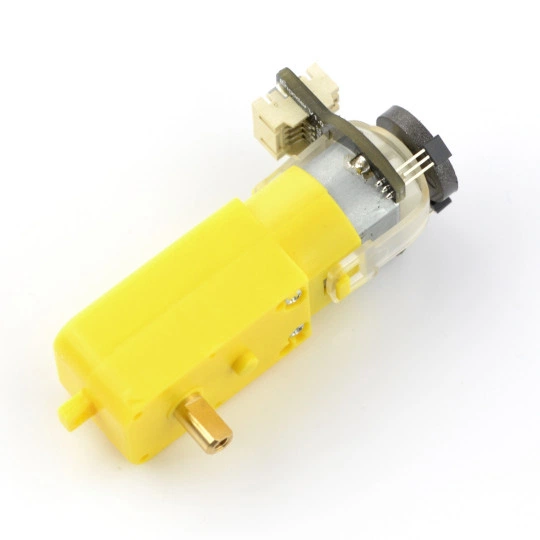
\includegraphics[width = 0.3\textwidth]{silnik_z_enkoder.png}
                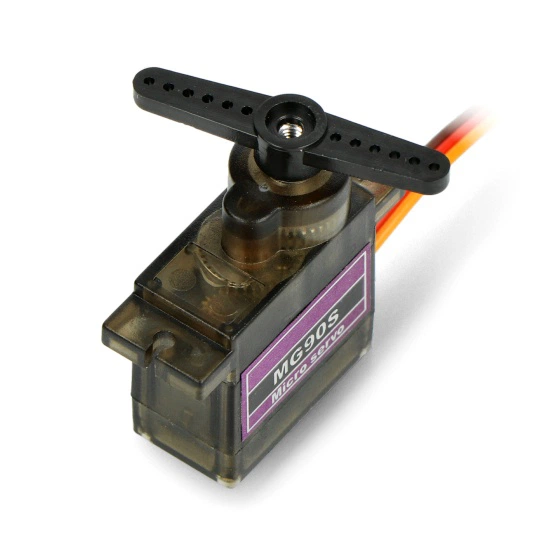
\includegraphics[width = 0.3\textwidth]{serwo_180.png}

                \caption{Silnik DC z enkoderem oraz serwomechanizmy $180^\circ$.}
                \footnotesize{Źródło: \href{https://botland.com.pl/}{botland.com}}
                % Źródło: https://botland.com.pl/silniki-dc-z-przekladnia-i-enkoderami/6287-silnik-z-przekladnia-sj01-120-1-6v-160rpm-enkoder-6959420910205.html
                % Źródło: https://botland.com.pl/serwa-typu-micro/20435-serwo-mg-90s-micro-180-stopni-metalowa-przekladnia-5904422380915.html
                \label{fig:engines}
            \end{figure}

        \subsubsection{Pomiar odległości}
            Autonomia pojazdu, nie ogranicza się wyłącznie do sterowania silnikami.
            Pojazd tego typu musi być świadomy swojego otoczenia. Ta funkcja wymaga wykorzystania czujników pozwalających na pomiar odległości.
            Poniżej przedstawiono listę różnych rodzajów czujników:
            \begin{enumerate}
                \item Czujnik ultradźwiękowy -- najpopularniejsze układy wykorzystywane do pomiaru odległości.
                Natomiast ich pomiary bywają niestabline. Ich zaletą jest prostota działania, jednak okupiona jest ona długim czasem wykonywania pomiarów.
                \item Czujniki Time of Flight (ToF) -- złożone, wyspecjalizowane moduły z dużą dokładnością, pozwalające osiągnąć bardzo daleki zasięg pomiarowy.
                Zazwyczaj wymagają specjalnych bibliotek dostarczonych przez producenta, co stanowi zarówno wadę jak i zaletę. Takie czujniki mogą być bardzo szybkie, jednak złożona, uniwersalna biblioteka, znacząco spowalnia ich pracę.
                \item Układy obiciowe IR(wytłumaczenie) -- układ składający się z dwóch diod, emitera i odbiornika. Cechuje się niewielkim zakresem pomiarowym (od $2cm$ do $20cm$) i małą jego dokładnością (pomiar zależy od koloru obiektu) oraz dużą strefą martwą.
                \item Lidar -- wyspecjalizowane układy, pozwalające na bardzo precyzyjny pomiar w pełnym zakresie $360^\circ$.
                Sprawia to że jest jedną z najlepszych dostępnych opcji, jednak ceny takich układów są zaporowe.
                \item Radar -- bardzo dokładne i kosztowne układy pomiarowe, pozwalające na niezwykłą precyzję. Niestety, ich rozmiar wymagady do tego projektu jest trudo dostępny na rynku konsumenckim. Dodatkowo, wymagają specjalnych procesorów sygnałowych pozwalających na bieżąco przetwarzać dane z radarów.
            \end{enumerate}
            Z przedstawionej listy, układami które sprawdzą się najlepiej w tym projekcie są czujniki typu ToF, zamontowane z przodu pojazdu.
            Dodatkowo, ze względów bezpieczeństwa, z tyłu zamontowane zostały czujniki IR. Natomiast, nie są one wykorzystywane jako urządzenia pomiarowe,
            tylko jako czujniki zbliżeniowe, umożliwiające wykrycie przeszkody i reakcję na niebezpieczeństwo.

    \subsection{Środowisko programistyczne}
        Następnym bardzo ważnym wyborem jest środowisko programistyczne, w którym zostanie zbudowany projekt.
        Tutaj też w ostatnich latach użytkownicy dostali olbrzymie możliwość wyboru.
        Podstawowymi rozwiązaniami dla programistów embedded są:
        \begin{enumerate}
            \item Eclipse -- kiedyś bardzo popularny, posiadający olbrzymi zbiór dodatków.
            Jest także rozprowadzany na otwartej licencji dlatego stanowi świetną bazę dla wielu bardziej zaawansowanych projektów.
            \item STM32 Cube -- środowisko przeznaczone strike do pracy z modułami STM32, oparte na Eclipsie.
            \item Atmel Studio -- środowisko przeznaczone do pracy z mikrokontrolerami z rodziny AVR od firmy ATmel.
            \item Keil µVision -- środowisko ogólnego przeznaczenia do pracy z układami Cortex, ograniczone licencją.
            \item Notepad++ -- bardziej zaawansowany notatnik, pozwalający na auto uzupełnianie słów. Na też masę wtyczek, pozwalających na stworzenie z niego pełnoprawnego środowiska programistycznego, jednak w swojej pierwotnej wersji bardzo trudny w użyciu.
            \item VS Code -- bardzo uniwersalne narzędzie, mające olbrzymią masę dodatków, pozwalających przystosować środowisko w pełni pod własne wymagania.
            Samo środowisko jest zbudowane na silniku przeglądarki internetowej, dzięki czemu może z powodzeniem zastąpić przeglądarkę PDF, a w wbudowany tile menedżer pozwala układać całość w bardzo czytelny sposób.
        \end{enumerate}
        Projekt został, zbudowany w środowisku VS Code, ze względu na największą elastyczność oraz możliwość dostosowania go do własnych potrzeb.


    \subsection{Środowisko CAD}
        Zbudowanie pojazdu autonomicznego wymaga wymodelowania odpowiednich części.
        % Dodatkowo, praca wymagała zaprojektowania kilku dodatkowych elementów mechanicznych.
        W tym celu, zostało wykorzystane środowisko CAD, które pozwala na zbudowanie modelu 3D.
        Poniżej przedstawiono listę kilku najpopularniejszych programów do projektowania.
        \begin{enumerate}
            \item SolidWorks -- program stworzony przez firmę Dassault Systemes, który jest bardzo popularny w przemyśle. Jest też niezwykle precyzyjny i każda operacja wymaga zastanowienia się dokładnie co chce się osiągnąć - przez co próg wejścia jest bardzo wysoki.
            \item Fusion 360 -- program stworzony przez firmę Autodesk, przeznaczony specjalnie do modelowania 3D. Posiada olbrzymie wsparcie dla drukarek 3D, a także dla obrabiarek CNC.
                                Jest także niezwykle intuicyjny a próg wejścia jest bardzo niski. Jedyną wadą programu, jest możliwość jedynie pracy w chmurze.
            \item FreeCAD -- darmowy program do projektowania modeli 3D, bardzo prosty w obsłudze, a nauczenie się tego programu wymaga naprawdę niewielkiego wkładu pracy.
                             Program jest stale rozwijany, a społeczność wokół niego ma możliwość rozbudowywania go o nowe funkcje. Niewątpliwą zaletą w porównaniu do innych programów jest możliwość uruchomienia go na każdym systemie operacyjnym.
        \end{enumerate}

        W projekcie został wykorzystany program FreeCAD, ze względu na swoją prostotę oraz możliwość uruchomienia na systemie Linux.


        \useNormalLandscape
\section{Schemat blokowy}
    Na schemacie blokowym \ref{schema:block}, przedstawiono przepływ sygnałów sterujących, wraz z poszczególnymi blokami.
\begin{figure}[!ht]
\centering
\vspace{1cm}
\begin{circuitikz}[fill = white]
    \draw[very thick]
        (0, 0) node[draw, rectangle, fill, minimum width = 4cm, minimum height = 4cm, align = center] (MCU) {Mikrokontroler\\\scriptsize{Raspberry PI PICO W}}

        (0, -5) node[draw, rectangle, fill, minimum width = 3cm, minimum height = 3cm, align = center] (HBridge){Mostek H}
        (HBridge.south) ++(1, 0) --++(0, -1) to[Telmech=M, n = LMotor] ++ (2, 0) --++ (0, 2) --++ (-2, 0)
        (HBridge.south) ++(-1, 0) --++(0, -1) to[Telmech=M,n = RMotor] ++ (-2, 0) --++ (0, 2) --++ (2, 0)

        (-10, 4) node[draw, rectangle, fill, minimum width = 2cm, minimum height = 2cm, align = center] (ToF1) {$\text{ToF}_1$}
        (-7, 4) node[draw, rectangle, fill, minimum width = 2cm, minimum height = 2cm, align = center] (ToF2) {$\text{ToF}_2$}
        (-4, 4) node[draw, rectangle, fill, minimum width = 2cm, minimum height = 2cm, align = center] (ToF3) {$\text{ToF}_3$}

        (-6, 0) node[draw, rectangle, fill, minimum width = 2cm, minimum height = 2cm, align = center] (MPU6050){MPU6050\\lub\\MPU6000}
        (-6, -4) node[draw, rectangle, fill, minimum width = 2cm, minimum height = 2cm, align = center] (Magneto){Magnetometr}

        (6, -4) node[draw, rectangle, fill, minimum width = 2cm, minimum height = 2cm, align = center] (LIR){Czujnik\\cofania}
        (9, -4) node[draw, rectangle, fill, minimum width = 2cm, minimum height = 2cm, align = center] (RIR){Czujnik\\cofania}

        (6, 4) node[elmech=M, scale = 1.5](servo){S}
        (8, 0) node[draw, rectangle, fill, minimum width = 2cm, minimum height = 2cm, align = center] (memory) {Pamięć}
    ;

    \draw[]
        (MCU.east) to[bmultiwire = 4, a = SPI] (memory.west)
        (MCU.east) ++ (0, 1) to[short, i=PWM] ++ (4, 0) -| (servo.south)
        (MCU.east) ++ (0,-1) to[bmultiwire = 2] ++ (2, 0) --++ (0, -1) to[short, i<= Detect, -*]++ (2, 0) coordinate(IR_node)
            (IR_node)  to[multiwire=1] (LIR.north)
            (IR_node)  to[multiwire=1] ++ (3, 0)-| (RIR.north)
    
        (MCU.south) to[tmultiwire=6, i=\ ] (HBridge.north)

        (MCU.west) to[bmultiwire = 2, a = I2C, -*] ++ (-2, 0) coordinate(I2C) 
        (I2C) -- (MPU6050.east)
        (I2C) |- (Magneto)

        (I2C) to[short, -*] ++ (0, 2) coordinate(I2C)
        (I2C) -- (ToF3.south)
        (I2C) to[short, -*]++ (-3, 0) coordinate(I2C) -- (ToF2.south)
        (I2C) -| (ToF1)

        (LMotor) to[crossing] ++ (0, 4) --++ (0, 0.5) to[bmultiwire, a = 2] ++ (-1, 0) --++ (0, 1)
        (RMotor) to[crossing] ++ (0, 4) --++ (0, 0.5) to[bmultiwire = 2] ++ ( 1, 0) --++ (0, 1)
    ;
\end{circuitikz}
\renewcommand{\figurename}{Schemat}
\caption{Schemat blokowy, przedstawiający przepływ sygnałów w projekcie}
\label{schema:block}
\end{figure}
    \useportrait
% \footnote{Pamięć dodatkowa do przechowywania map terenu}

    \section{Środowisko testowe}
\label{sec:testing}
    Podczas budowy dowolnego systemu, niezwykle ważne jest testowanie elementów składowych każdego z bloków.
    W informatyce testowanie oprogramowania zapewniają testy jednostkowe, które sprawdzają działanie poszczególnych algorytmów i programów.
    W przypadku prac nad hardwarem niezbędne jest zbudowanie odpowiedniego środowiska, pozwalającego na testowanie każdego elementu osobno oraz łącznie z innymi elementami.
    % Dlatego przedstawiony projekt można podzielić na kilka części:
    Dlatego wykonanie fizyczne można podzielić na kilka części:
    \begin{enumerate}
        \item Budowa prototypu na płytce stykowej.
        \item Złożenie ramy pojazdu z elektroniką umieszczoną na płytce stykowej wraz z doprowadzonym zewnętrznym zasilaniem.
        \item Sprawdzenie działania pojazdu z płytką stykową zasilaną bateryjnie.
        \item Wykonanie płytki prototypowej z połączeniami wszystkich elementów na stałe ponownie z zewnętrznym zasilaniem.
        \item Sprawdzenie działania prototypu pojazdu z zasilaniem akumulatorowym.
    \end{enumerate}
    Każdy z wymienionych etapów charakteryzował się innym rodzajem testów oraz własnymi problemami.
    Zakończenie jednej fazy i przejście do następnej, było możliwe dopiero po uznaniu przez autora, że układ pracuje poprawnie.

    \subsection{Modele prototypowe}
        Pierwszym krokiem, było zbudowanie na podstawie schematu \ref{schema:block} modelu elektronicznego na płytce stykowej.
        Poniżej przedstawiono zdjęcie układu złożonego w ten sposób.
        Obwód ten pozwalał na bezpieczne testowanie nowych funkcji, bez ryzyka uszkodzenia elementów.
        Dodatkowymi zaletami takiego połączenia, są: możliwość bezpośredniego debugowania kodu, a także możliwość szybkiej zmiany połączeń w przypadku konfliktów między podzespołami.
        \begin{figure}[!ht]
            \centering
            \includegraphics[width = 0.7\textwidth, trim = {500px, 500px, 350px, 350px}, clip]{Breadboard.jpg}
            \caption{Model prototypowy na płytce stykowej}
            \label{fig:breadboard}
        \end{figure}

        Model z płytki stykowej, został skompresowany aby zmieścił się na pojedynczej płytce o rozmiarach 400-stu pól.
        Tak ściśnięty układ można było założyć na ramę pojazdu.
        W tym celu zaprojektowano i wydrukowano niedużą podporę, która pozwoliła na sztywne zamocowanie układu.

        \begin{figure}[!ht]
            \centering
            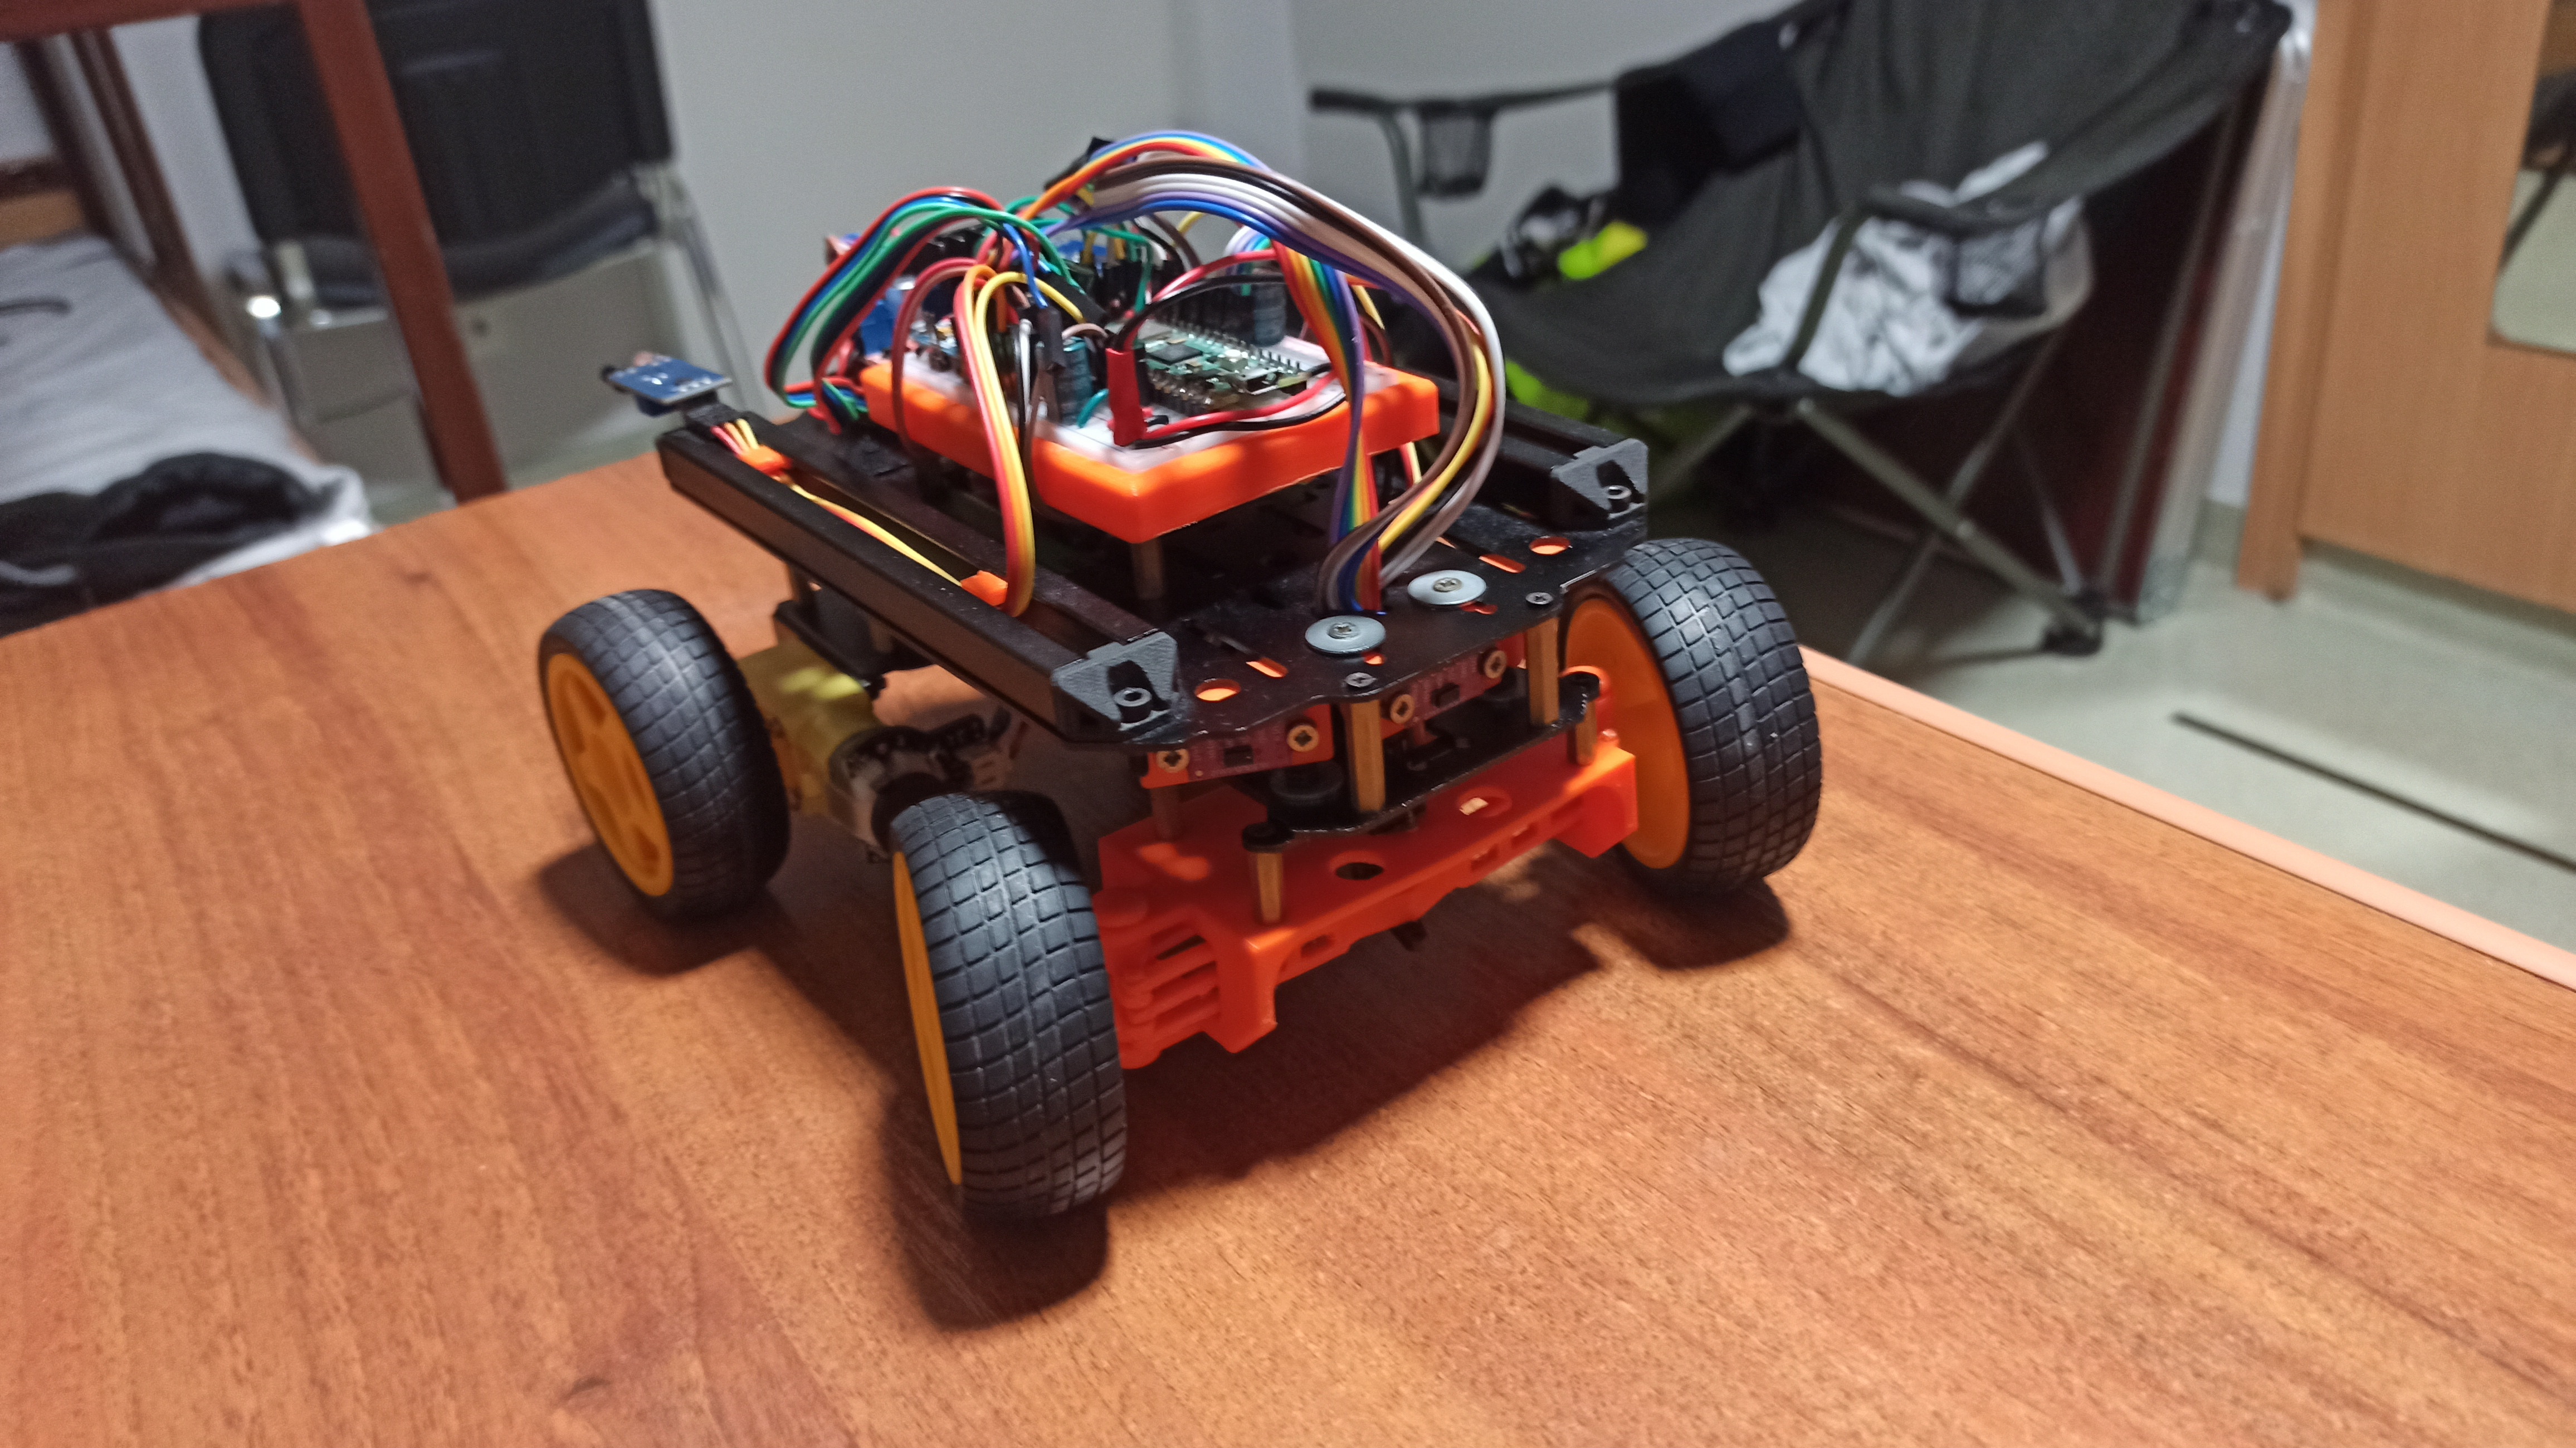
\includegraphics[width = 0.7\textwidth, trim = {800px, 400px, 1200px, 200px}, clip]{Breadboard_car.jpg}
            \caption{Model pojazdu z zainstalowaną płytą stykową}
            \label{fig:breadboard_car}
        \end{figure}

        Po zamocowaniu płytki do ramy, pojazd został poddany testom jednostkowym.
        Testy te polegały na sprawdzeniu działania wszystkich komponentów.
        Następnie sprawdzono działanie podstawowych funkcji takich jak: jazda czy skręcanie.

        Podczas testowania elementów pojedynczo, wszystko działało poprawnie.
        Natomiast po dłuższym czasie testy wykazały, że układ akcelerometru, potrafi zawiesić się w przypadkowym momencie.
        Dodatkowo czasami, mikrokontroler przestawał reagować na polecenia.

        Problematyczna okazała się linia $SDA$ protokołu $I^2C$.
        Rozwiązanie tego problemu było trudnym zadaniem.
        Szczególnie że bardzo ciężko było wykryć pierwotną przyczynę zawieszania się całego systemu.
        Pierwszą próbą rozwiązania problemu, było zastosowanie się do instrukcji z noty aplikacyjnej od Analog Devices o resetowaniu linii $I^2C$ \cite{application_note_I2C_AD}.
        Podobne rozwiązanie można znaleźć w dokumentacji do magistrali $I^2C$ \cite{I2C_manual_NXP} wydanej przez NXP.
        Niestety, zastosowane rozwiązanie nie przyniosło oczekiwanych rezultatów.

        Drugim rozwiązaniem sugerowanym przez oba dokumenty, w sytuacji kiedy nie udało się odblokować magistrali jest zresetowanie niedziałających (w domyśle wszystkich) układów.
        To rozwiązanie, mimo swojej skuteczności nie zostało wykorzystane, ze względu na bardzo długo czas ponownej inicializacji wszystkich czujników.
        Autor skupił się na znalezieniu pierwotnej przyczyny problemu, którą okazała się płytka stykowa.
        Podczas jazdy, cały pojazd drżał, co powodowało, że niektóre piny nie stykały i układ akcelerometru, po spadku zasilania, blokował magistralę $I^2C$.
        Rozwiązaniem tego problemu, w tej wersji projektu, okazało się niemożliwe, ze względu na działanie zastosowaną metodę połączeń.

        Niespodziewaną zaletą wykonania w pierwszej wersji projektu na płytce stykowej oraz losowego zawieszania się programu, było udoskonalenie funkcji odpowiedzialnych za kontrolę protokołu $I^2C$.
        W pierwszej wersji programu, komunikacja $I^2C$, blokowała pracę procesora.
        Rozwiązanie to sprawdzało się tak długo jak wszystko działało poprawnie.
        Jednak luźne połączenia ukazały, że jest to niepraktyczne.
        W poprawionej wersji programu dla Raspberry, instrukcje odpowiedzialne za komunikację $I^2C$ zostały ograniczone \textit{timeoutem} dzięki czemu, procesor nie zawieszał się w przypadku braku odpowiedzi od czujnika.

        Ostateczną wersją prototypu jest zlutowana na stałe płytka prototypowa.
        To połączenie układu pozwoliło pozbyć się niektórych problemów, przykładowo blokowania się magistrali $I^2C$.
        Jednak zlutowana wersja objawiła inne problemy, które ukrywała płytka stykowa.
        \begin{figure}[!ht]
            \centering
            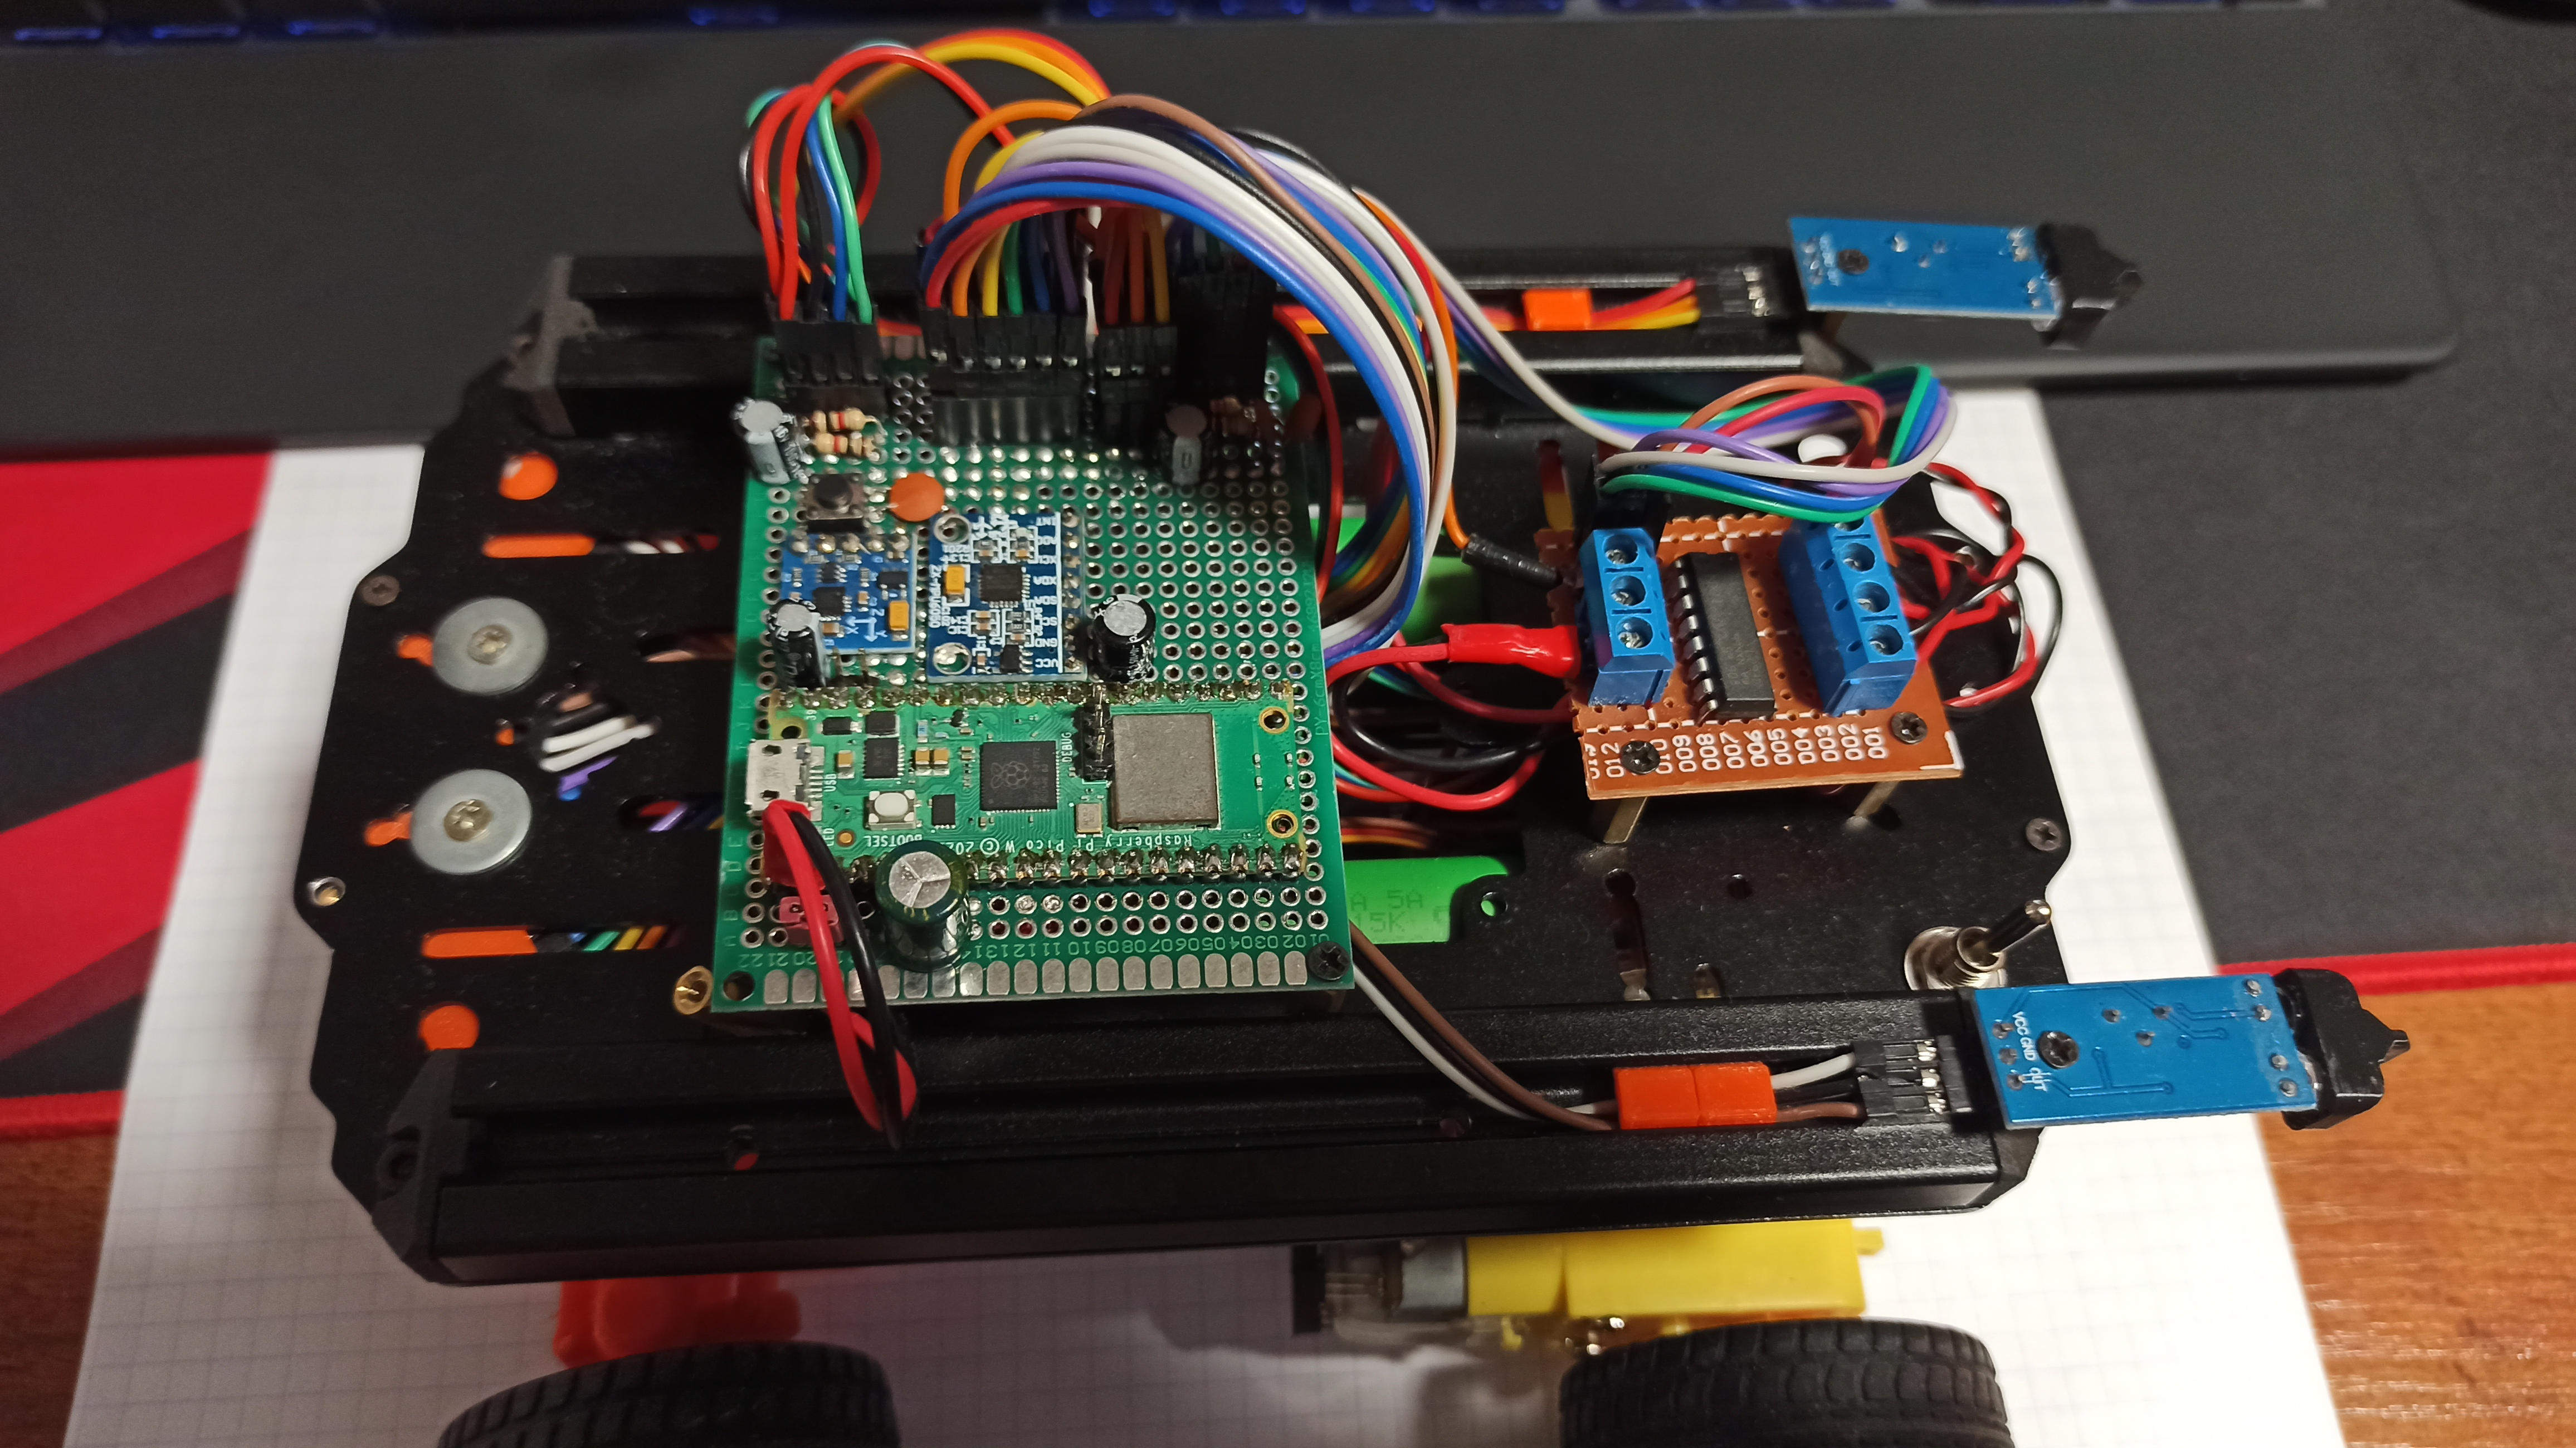
\includegraphics[width = 0.7\textwidth, trim = {500px, 300px, 300px, 200px}, clip]{Protoboard_car.jpg}
            \caption{Model pojazdu z zainstalowaną płytą prototypową}
            \label{fig:protoboard_car}
        \end{figure}

        Największym problemem, który pojawił się podczas testowania tej fazy, było losowe resetowanie się RPi Pi (Raspberry Pi).
        Znalezienie przyczyny takiego zachowania również nie było łatwym zadaniem.
        Problem występował czasami zarówno po podłączeniu zewnętrznego zasilacza jak i pracy na akumulatorach.
        Po testach okazało, się że sytuacja ta występuje tylko wtedy, gdy pracują silniki oraz podłączone są enkodery.
        Po odłączeniu wyjść sygnałowych enkoderów, kłopot z resetowaniem się układu zniknął.
        W celu upewnienia, się że przyczyną są uszkodzone enkodery, w szereg z wyjściem sygnałowym został podłączony rezystor o rezystancji $R =1k\Omega$, które chroniły układ przed zwarciem.
        Po podłączeniu rezystora, problem z resetowaniem się układu zniknął na kilka dni, po czym powrócił.
        Szukając problemów w okolicy silników, zostało zmienione zasilanie silników na niezależne od reszty układu.
        Uruchomienie silników, z zasilaniem niezależnym natychmiast zresetowało procesor.
        Kolejną próbą była zmiana mostka H na inny. Wymiana tego układu również nie pomogła.
        W między czasie podczas składania prototypu, uszkodzeniu uległ jeden z układów ToF.
        Po wymianie uszkodzonego układu, problem z resetowaniem się RB Pi Pico nie zniknął.
        Ostatnim pomysłem co mogło zostać uszkodzone, była sama malinka, jednak jej wymiana również nie pomogła.
        Ostatecznie, rozwiązaniem okazało się dołożenie dużej roznoszonej pojemności (około $500\mu F$) na całej płytce.

        Kolejnym problemem, na który natrafił autor, były oscylacje na liniach przerwań od czujników obiektów zamontowanych na tyle pojazdu.
        Oscylacje te, nie pozwalały na poruszanie się do tyłu, ponieważ czujniki w losowych momentach zgłaszały obiekt i zatrzymywały silniki.
        Rozwiązaniem tego problemu było zastosowanie filtru RC, który niweluje drgania.



    \subsection{Automatyzacja praca}
        Automatyzacja pracy jest niezwykle ważnym zadaniem w momencie, testowania podstawowych funkcji.
        Oczywiście, każdą funkcję można wywołać ręcznie, jednak podczas testów, kiedy wielokrotnie wykonywane są podobne funkcje, automatyzacja staje się obowiązkowa.

        Aby wykonać to zadanie, w języku Python został napisany skrypt, który pozwala na dwustronną komunikację za pomocą protokołu $UDP$.
        Dodatkowo, program pozwala na interpretację plików, napisanych specjalnie dla tego układu.
        Poniżej przedstawiono listing \eqref{list:self_test.s} programu do testowania podstawowych działań pojazdu.

        \lstinputlisting[style=asm, caption={Test pojazdu}, label = list:self_test.s]{Listing/self_test.s}

        \subsubsection{Interpreter własnego języka}
            Przedstawiony w listingu \ref{list:self_test.s} program jest interpretowanym przez skrypt napisany w pythonie.
            Jego zadaniem jest stokenizowanie instrukcji, wyznaczanie adresów skoków oraz stworzenie słownika z zmiennymi.
            Następnie, program przechodzi do wykonywania instrukcji zapisanych w pliku.
            Powyższy język posiada tylko kilka prostych słów kluczowych przedstawionych w tabeli \ref{table:keywords}.
            Pozostałe instrukcje po sformatowaniu wysyłane są do malinki.

            \begin{table}[!ht]
                \centering
                \caption{Lista słów kluczowych do mini języka}
                \begin{tabularx}{0.8\textwidth}{|c|c|C|}\hline
                    Nr. & Instrukcja & Opis \\\hline
                     1. & jump $etykieta$ & Skok do $etykiety$ \\\hline
                     2. & end & Koniec programu lub funkcji \\\hline
                     3. & print $zmienna/napis$ & Wypisanie wartości zmiennej lub napisu\\\hline
       \centerY{2}{ 5.} & \centerY{2}{if $warunek$} & Instrukcja warunkowa, w przypadku nie spełnienia pomija następną instrukcję\\\hline
       \centerY{2}{ 7.} & \centerY{2}{$etykieta$\textbf{:}} & Etykieta funkcji, koniecznie zakończona znakiem ,,:''\\\hline
       \centerY{4}{ 9.} & \centerY{4}{$\$zmienna$} & Odwołanie do zmiennej w przypadku instrukcji wysłanych. Podczas formatowania instrukcje, $\$zmienna$ zostaje podmieniona na wartość\\\hline
       \centerY{2}{10.} & \centerY{2}{$zmienna$ = \textit{wartość}} & Przypisanie wartości do zmiennej. Pozwala na wykonywanie operacji matematycznych\\\hline
                \end{tabularx}
                \label{table:keywords}
            \end{table}

            Wszystkie pozostałe instrukcje, które nie są zdefiniowane w tabeli, wysyłane są bezpośrednio do mikrokontroler.
            Natomiast w przypadku, kiedy instrukcja zostaje odnaleziona, ale zawiera błąd składniowy, program wyświetla błąd i przerwa działanie.
            Przykład takiej sytuacji przedstawiono na rysunku \ref{fig:interpreter}.

            \begin{figure}[!ht]
                \centering
                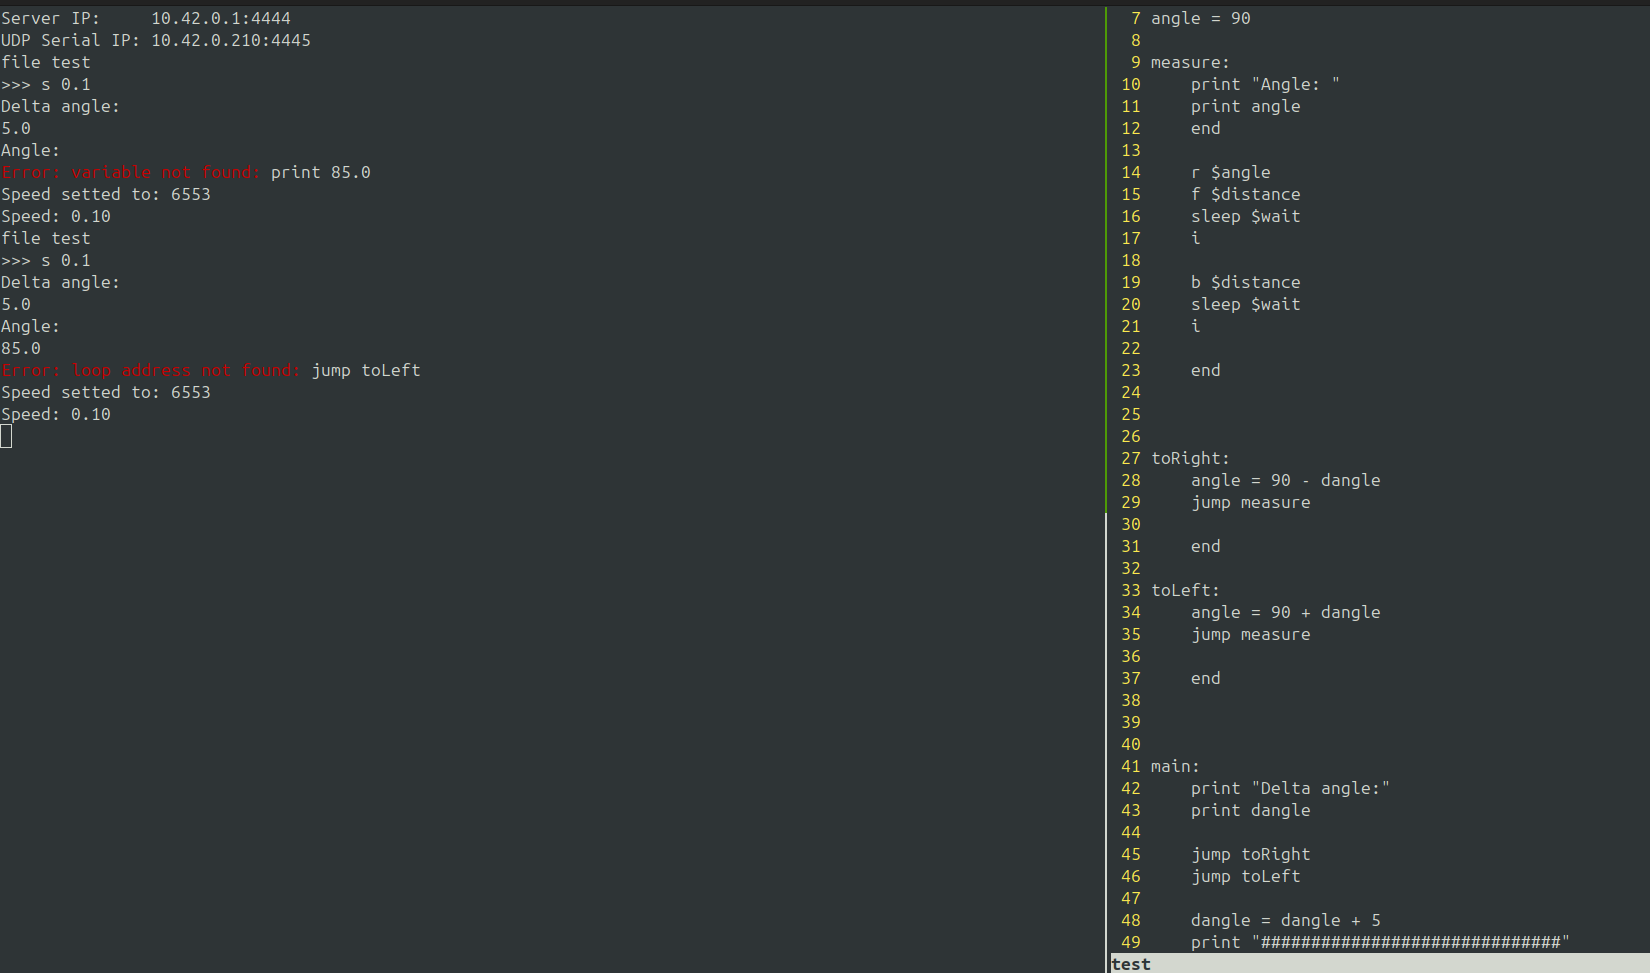
\includegraphics[width = 0.7\textwidth]{Terminal_program_testowy.png}
                \caption{Program zawierający celowe błędy}
                \label{fig:interpreter}
            \end{figure}

            W przypadku, kiedy program pracuje poprawnie, instrukcje wypisywane są równolegle z wiadomościami odebranymi od samochodu.
            Rozkazy wysyłane do mikrokontrolera, są poprzedzone łańcuchem znaków ,,$>>>$''.
            Natomiast instrukcja wynik instrukcji $print$ jest identyczny z tym, co zwraca mikrokontroler.
            Podczas testowania programy, program zdążył wysłać kilka instrukcji do raspberry dlatego po zgłoszeniu błedy widnieją widnieje kilka odebranych instrukcji.
    \section{Budowa pojazdu - założenia i testy}
    Inspiracją do stworzenia poniższego projektu, były samochody autonomiczne, które najczęściej są pojazdami dwuosiowymi, o jednej osi skrętnej i jednej osi napędzającej.
    Obie osie, nie będą połączone ze sobą, co pozwoli na niezależne sterowanie nimi.
    W projekcie zostaną użyte dwa silniki prądu stałego wybrane w rozdziale \ref{sec:engines}.
    Silniki zostały podłączone bezpośredni do kół w osi tylnej.
    \subsection{Przednia oś}
        Przednia oś, została połączona układem kierowniczym, opartym na serwomechanizmie.
        Na rysunku \ref{fig:frontAxis_model} przedstawiono model tego układu zaprojektowanego przez autora.

        \begin{figure}[!ht]
            \centering
            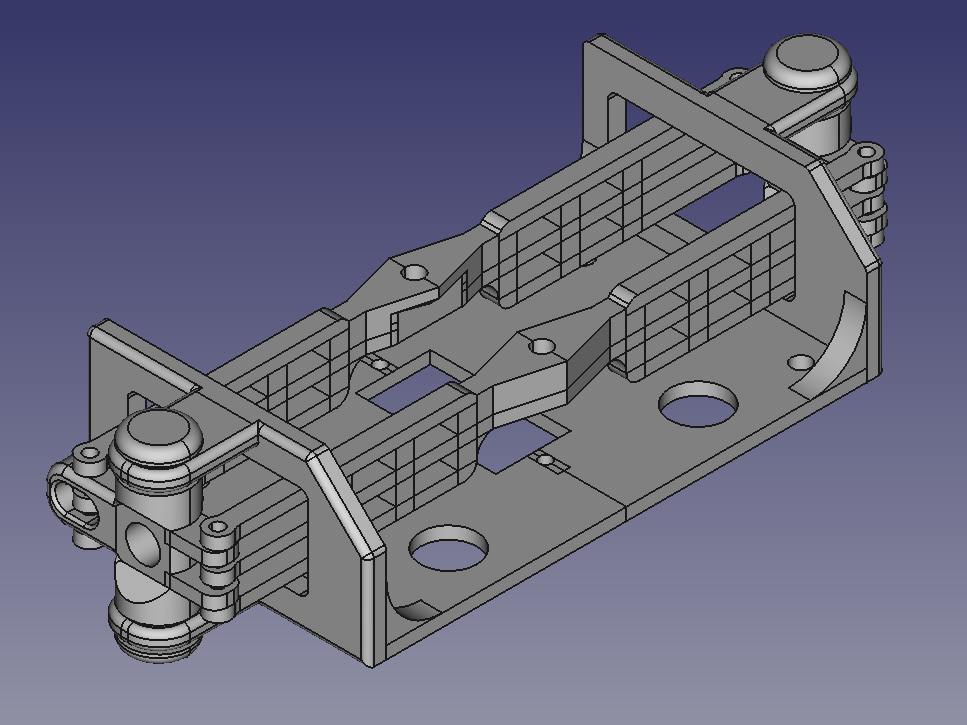
\includegraphics[width=0.7\textwidth]{FronAxis_example.png}
            \caption{Przykładowy układ kierowniczy zaprojektowany w narzędziu FreeCAD}
            \label{fig:frontAxis_model}
        \end{figure}
        Oś ta została zaprojektowana w taki sposób, aby środek kół znajdował się w linii z środkiem serwomechanizmu.
        Dzięki temu, kąt ustawienia serwomechanizmu, odpowiada kątowi skrętu kół.
        Natomiast dużą wadą takiego układu, jest brak możliwości odczynia aktualnej pozycji kół, które po osiągnięciu swojego limitu mogą zniszczyć serwo.

    \subsection{Rama pojazdu}
    Na czas beta testów, został wykorzystana gotowa rama przedstawiona na zdjęciu \ref{fig:test_chassis}.
    \begin{figure}[!ht]
        \centering
        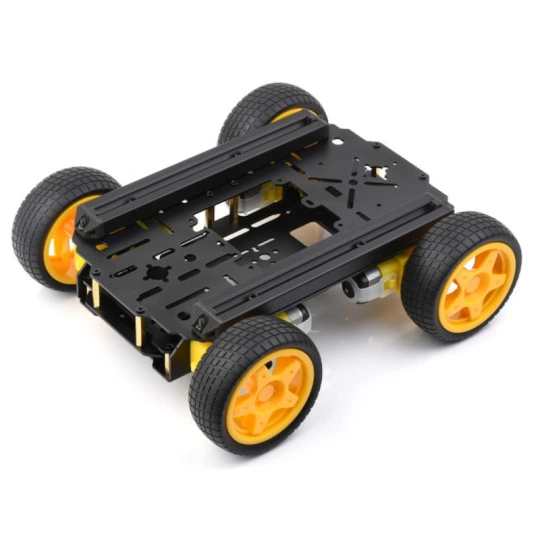
\includegraphics[width=0.7\textwidth]{chassis-waveshare-24419.png}
        \caption{Rama testowa Waveshare 24419}
        Źródło: \citetitle{chassis_waveshare} \cite{chassis_waveshare}
        \label{fig:test_chassis}
    \end{figure}

    Rama wstępnie została przerobiona aby możliwe było sterowanie przednią osią. Zgodnie z zdjęciem \ref{fig:frontAxis_model}.
    Dodatkowo, został zmieniony sposób montażu silników, które zostały zamocowane na odwrotnie do zaleceń producenta, a także, zrezygnowano z ,,gumek", odpowiadających za amortyzację.


    % TODO: dodać opis ramy pojazdu

    \subsection{Pomiar odległości}
        Pomiar odległości jest podstawową funkcjonalności, współczesne pojazdy autonomiczne wykorzystują układy LIDAR, które pozwalają mierzyć pełne $360^\circ$.
        Jednak w wielu sytuacjach taki pomiar mija się z celem, gdyż znaczna większość próbek zostaje odrzucona.
        Same lidary, zaś są bardzo drogimi urządzeniami, często z niestandardowym sposobem komunikacji (np. za pomocą UART). 
        Dlatego, też autor, zdecydował się na zastosowanie tańszych czujników ToF.
        Trzy takie czujniki zostały zamocowane z przodu pojazdu, z rozstawieniem co $30^\circ$.
        Na rysunku \ref{fig:ToF_holder}, przedstawiono wyżej opisany sposób montażu.
% \newpage
        \begin{figure}[!ht]
            \centering
            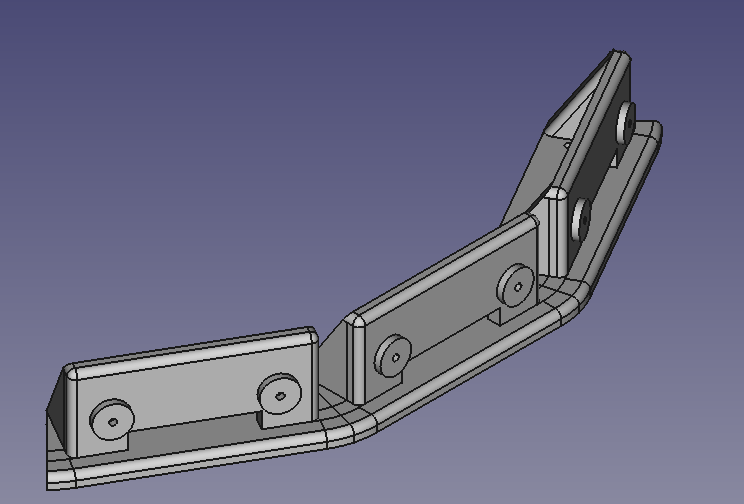
\includegraphics[width=0.7\textwidth]{ToF_holder.png}
            \caption{Mocowanie czujników ToF}
            \label{fig:ToF_holder}
        \end{figure}

    \section{Problemy konstrukcyjne}
\label{sec:problemy_konstrukcyjne}
    W poniższym rozdziale zostaną przedstawione problemy konstrukcyjne,
    które pojawiły się podczas realizacji projektu.

    \subsection{Jazda prosto}
        Najprostszą czynnością każdego pojazdu, jest jazda prosto.
        Operacja ta może wydawać się prosta, jednak wcale taka nie jest.
        Przykładowo, kiedy usiądziemy za kierownicą, prawdziwego samochodu, kontroluje podświadomie wiele parametrów takich jak:
        \begin{itemize}
            \item nachylenie terenu,
            \item aktualną pozycję kół,
            \item linie poziome na drodze czy pobocze drogi.
        \end{itemize}
        Jako ludzie, wiele tych parametrów kontroluje ,,na wyczucie" jednak pojazdy autonomiczne, są poniekąd robotami, dla których istnieje tylko informacja \textit{tak} lub \textit{nie}.
        Poniższy projekt podczas testów, wykazywał wiele mankamentów, które uniemożliwiały jazdę prostą.
        Były to między innymi:
        
        \subsubsection{Różnica prędkości silników}
            Zastosowanie dwóch silników, ma swoje wady i zalety.
            Olbrzymią zaletą jest możliwość zwiększenia mocy pojazdu.
            Jednak olbrzymią wadą okazało się sterowanie i nierównomierność pracy silników.
            Na wykresie \ref{plot:distance_err_in_time_const_speed} poniżej przedstawiono 

            \begin{figure}[!ht]
                    % TODO: zebrać pomiary odległości przebytej przez układ od czasu bez PID
                \centering
                \begin{tikzpicture}
                    \begin{axis}[
                        width = 0.7\textwidth,
                        grid = both,
                        grid style = dashed,
                        % axis lines = middle,
                        xlabel = czas ${[s]}$,
                        ylabel = różnica odległości ${[mm]}$,
                        xmin = 0,
                        xmax = 20,
                    ]
                        \addplot[blue] table[x = Time, y = Diff, col sep = comma]{Measure/distance_no_PID_speed_50.csv};
                        \legend{Błąd odległości}
                    \end{axis}
                \end{tikzpicture}
                \renewcommand{\figurename}{Wykres}
                \caption{Różnica przebytej drogi między prawym a lewym silnikiem bez regulacji}
                \label{plot:distance_err_in_time_const_speed}
            \end{figure}

            Aby rozwiązać powyższy problem należy zastosować regulator PID, pozwalający w trakcie pracy silników, na bieżąco korygować prędkość silników.
            Natomiast na samym początku ruchu została zastosowana sztywna korekta prędkości silników, w celu zminimalizowania błędu.
            \begin{figure}[!ht]
                \centering
                \begin{tikzpicture}
                    \begin{axis}[
                        width = 0.7\textwidth,
                        grid = both,
                        grid style = dashed,
                        % axis lines = middle,
                        xlabel = czas ${[s]}$,
                        ylabel = różnica odległości ${[mm]}$,
                        xmin = 0,
                        xmax = 60,
                    ]
                        \addplot[blue] table[x = Time, y = Distance_err, col sep = comma]{Measure/PID_speed_10.csv};
                        \legend{Błąd odległości}
                    \end{axis}
                \end{tikzpicture}
                \renewcommand{\figurename}{Wykres}
                \caption{Różnica przebytej drogi między prawym a lewym silnikiem z włączonym regulatorem PID. Prędkość pojazdu: $(17.60 \pm 0.10)\frac{mm}{s}$.}
                \label{plot:PID_distance_err_in_time}
            \end{figure}

            Jak widać na wykresie \ref{plot:PID_distance_err_in_time} w początkowej fazie, silniki nadal nie pracują równomiernie, w dłuższej perspektywie praca silników osypuje w okół stałej wartości $(0 \pm 3)mm$.

    \subsubsection{Nie idealność podwozia}
        Kolejnym napotkanym problemem, okazuje się nie idealność podwozia, szczególnie elementu przedstawionego na rysunku \ref{fig:frontAxis_model} oraz nie równomierne rozłożenie masy względem środka.
        Wszystkie wyżej wymienione niedokładności powodowały, że pojazd cały czas skręcał w jedną stronę.
        Rozwiązaniem tego problemu jest zastosowanie układy pętli zwrotnej, opartej na czujniku $MPU6050$, który został użyty jak żyroskop, pozwalający na pomiar biedzącego kąta.
        Dzięki czemu można korygować kierunek skręcania pojazdu.
        
        Jednak jego wykorzystanie nie było bezproblemowe i wymagało dodatkowych poprawek.
        Na wykresie \ref{plot:gyro_magneto_measure} przedstawiono pomiar kąta dla obrotu pojazdu ze stałą prędkością w jednym kierunku.
        Poniższy pomiar został wykonany w celu ustalenia liniowości pracy żyroskopu opartego na akcelerometrze. 
        Układem referencyjnym był uprzednio skalibrowany magnetometr (układ $QMC5883L$).
% 
        \begin{figure}[!ht]
            \centering
                \begin{tikzpicture}
                    \begin{axis}[
                        width = 0.7\textwidth,
                        grid = both,
                        grid style = dashed,
                        xlabel = czas ${[s]}$,
                        ylabel = kąt zmierzony podczas obrotu ${[^\circ]}$,
                        ymin = -5,
                        ymax = 365,
                        xmin = 0,
                        xmax = 2.9,
                        ytick = {0, 30, ..., 360},
                        legend style={at={(0.2, 0.92)}, anchor=north},
                    ]
                        \addplot[orange] table[x = Time, y = Compass_azimuth, col sep = comma]{Measure/angles.csv};
                        \addplot[blue] table[x = Time, y = Gyro_z, col sep = comma]{Measure/angles.csv};
                        \legend{magnetometr,żyroskop}
                    \end{axis}
                \end{tikzpicture}
                \renewcommand{\figurename}{Wykres}
                \caption{pomiary azymutu za pomocą magnetometru, oraz zmiany kąta wykazanego przez żyroskop.}
                \label{plot:gyro_magneto_measure}
        \end{figure}
        Podczas pomiaru, na oba układy został nałożony filtr dolnoprzepustowy, eliminujący szumy.

        Wykres \ref{plot:delta_angle_with_gyro}, przedstawia narastanie katą, mierzonego przez żyroskop.
        Widać bardzo dużą liniowość pracy żyroskopu, co pozwala zaufać temu czujnikowi na tyle, aby na jego podstawie określać czy pojazd jedzie prosto.

        % \begin{wrapfig}[!ht]
        \begin{figure}[!ht]
            \centering
                \begin{tikzpicture}
                    \begin{axis}[
                        width = 0.7\textwidth,
                        grid = both,
                        grid style = dashed,
                        xlabel = czas ${[s]}$,
                        ylabel = kąt zmierzony podczas obrotu ${[^\circ]}$,
                        xmin = 0,
                        xmax = 2.9,
                    ]
                        \addplot[blue] table[x = Time, y = Delta_angle, col sep = comma]{Measure/angles.csv};
                    \end{axis}
                \end{tikzpicture}
                \renewcommand{\figurename}{Wykres}
                \caption{narastania kąta, zmierzonego przez żyroskop}
                \label{plot:delta_angle_with_gyro}
        \end{figure}
        % \end{wrapfig}


    \newpage
    Oba wyżej opisane rozwiązania pozwalają na w miarę stałą jazdę prostą.
    A w sytuacjach, kiedy pojazd zaczyna znacząco skręcać, na przykład po impakcie z boku, sprzężenie zwrotne z żyroskopu pozwala na w miarę łagodny powrót do oczekiwanego kąta.

    \subsection{Skręcanie}
        Rozwiązanie problemów z jazdą prosto to tylko połowa sukcesu.
        Kolejnym problemem okazało się skręcanie. 
        Nie tylko w pierwotnej wersji nie było stałe, ustawienie stałego kąta kół oraz przejechanie tej samej drogi, nie zawsze dawało ten sam rezultat.
        To pojazd cały czas miał tendencję do preferowania skrętu w jedną stronę.
        
        \subsubsection{Dyferencjiał}
        Najprostszym do zauważenia problemem był brak dyferencjału. 
        Tylna oś pojazdu posiadała dwa silniki, jednak w poprzednich testach, zostały one ,,software'owo połączona sztywną belką".
        Wyznaczenie wartości dyferencjału jest prostym zadaniem. Poniżej przedstawiono schemat algorytmu, na którego podstawie wyznaczono procentową wartość dyferencjału.
        Rysunek \ref{fig:turning_car}, przedstawia schematyczną sytuację skrętu pojazdu.-
        \begin{figure}[!ht]
    \centering
    \begin{tikzpicture}
        \draw
            (0, 0) node[draw, rectangle, rounded corners, fill = black, minimum width = 2cm, minimum height = 0.8cm, rotate = 30](frontL){}
            (0, -3) node[draw, rectangle, rounded corners, fill = black, minimum width = 2cm, minimum height = 0.8cm, rotate = 30](frontR){}

            (6, 0) node[draw, rectangle, rounded corners, fill = black, minimum width = 2cm, minimum height = 0.8cm](backL){}
            (6, -3) node[draw, rectangle, rounded corners, fill = black, minimum width = 2cm, minimum height = 0.8cm](backR){}

            (3, 0) node[above]{Zewnętrzna strona}
            (3,-3) node[below]{Wewnętrzna strona}
        ;

        \draw[Stealth-Stealth]
            (frontL) ++ (0, 1) --node[above]{$l$}++ (6, 0)
        ;
        \draw[dashed, gray]
            (frontL) --++(0, 1)
            (backL) --++(0, 1)
        ;

        \draw[color = red]
            (backL) -- ++ (0, -10) -- ++ (0, -1) coordinate(meet) --++ (0, -1)
            (frontL) -- (meet)
            (frontR) -- (meet)
        ;
        \draw
            (meet) ++ (0, 3) arc(90:127:3) node[above]{$\alpha$}
            (meet) ++ (0, 2) arc(90:147:1) node[above]{$\beta$}
        ;

        \draw[dotted]
            (backL) to[short, l=$\Delta r$] (backR)
            (backR) ++ (0, -2.5) node[right]{$r$}
        ;

        \draw[dashed]
            (frontL) ++ (0, 1) -- (0, -5)
            (0, -4) arc(90:180:-1)
            (0.5, -4.5) node[]{$\gamma$}
            (1.2, -4.25) node[rotate = -50]{$90 - \gamma$}
        ;
    \end{tikzpicture}
    \caption{Rysunek poglądowy do skręcenia}
    \label{draw:turning_car}
\end{figure}

        Jak widać na powyższym rysunku, skręt pojazdu można opisać jako ruch po kręgu, w którym poszczególne prędkości liniowe nie są sobie równe.
        Jednak występuje zależność:
        \begin{gather}
            \omega_{\text{lewe koła}} = \omega_{\text{prawe koła}}\\
            \frac{v_{\text{lewe koła}}}{r} = \frac{v_{\text{prawe koła}}}{r + \Delta r}\\
            \frac{v_\text{lewe koła}}{v_{\text{prawe koła}}} = \frac{r}{r + \Delta r}
        \end{gather}
        Jedynymi wartościami jakie są znane to:
        \begin{itemize}
            \item $l = 135mm$ -- długość między osiami samochodu:,
            \item $\Delta R = 155mm$ -- odległość między kołami w jednej osi,
            \item $\gamma \in <-30^\circ \div 30^\circ>$ -- kąt skrętu kół, ustawiany przez algorytm pathfinding'u lub użytkownika.
        \end{itemize}
        Dla powyższych parametrów, można wyznaczyć następującą równania:
        \begin{gather}
            \tan \left(90 - \gamma\right) = \frac{l}{r}
        \end{gather}
        Na podstawie powyższego równania można wyznaczyć funkcję długości promienia skrętu od aktualnego kąta, oraz 
        \begin{gather}
            r(\gamma) = \frac{l}{\tan(90-\gamma)}
        \end{gather}
        A zatem procentowy stosunek prędkości w funkcji kąta można wyznaczyć jako:
        \begin{gather}
            \frac{v_{\text{prawe koła}}}{v_{\text{lewe koła}}} = 1 + \frac{\Delta r}{r} = 1 + \Delta r \cdot \frac{\tan(90 - \gamma)}{l}
        \end{gather}

    \section{Sterowanie pojazdem}
    Sterowanie pojazdem powinno odbywać się w sposób płynny i precyzyjny.
    W poniższym rozdziale zostaną omówione algorytmy, odpowiedzialne za najbardziej podstawowe funkcje poruszania się takie jak: jazda prosto, skręt oraz cofanie.

    \subsection{Jazda przez pewien odcinek}
    \label{subsec:jazda_przez_odcinek}
        W rozdziale \ref{section:jazda_prosto}, zostały opisane problemy jakie wystąpiły podczas budowy pojazdu. %oraz problemy jakie musiały zostać rozwiązane aby samochód był w stanie jechać prosto.
        Dzięki rozwiązaniu wyżej wymienionych problemów, pojazd był w stanie jechać prosto.
        Jednak dla precyzyjnego sterowania, informacja o tym, że pojazd porusza po linii prostej, jest niewystarczająca.
        Obowiązkowym jest poznanie odległości jaką pokonuje pojazd.

        Dystans jaką pokonuje pojazd od momentu startu, możemy dość dokładnie obliczyć, korzystając ze wzoru \eqref{eq:pulseToDistance}.
        \begin{gather}
            s = \frac{\text{pulse} \cdot 2\pi R}{N}
            \label{eq:pulseToDistance}
        \end{gather}
        gdzie:
        \begin{itemize}
            \item $s$ -- odległość jaką pokonał pojazd,
            \item $\text{pulse}$ -- liczba impulsów z enkodera,
            \item $R$ -- promień koła,
            \item $N$ -- liczba impulsów na obrót koła.
        \end{itemize}

        Wzór ten, można także przekształcić w drugą stronę, aby obliczyć ile impulsów enkodera musi zostać zliczonych, przez procesor aby pojazd pokonał zadaną odległość.
        \begin{gather}
            \text{pulse} = \frac{s \cdot N}{2\pi R}
            \label{eq:distanceToPulse}
        \end{gather}

        Dla zbudowanego modelu, promień koła wynosi $R = 50cm$, a liczba impulsów zgodnie z dokumentacją wynosi $N = 1920$.
        A więc dokładność pomiaru odległości wynosi około:
        \begin{gather}
            \Delta s \approx \pm2.0mm
        \end{gather}

        Dzięki zastosowaniu równania \eqref{eq:distanceToPulse}, możliwe jest wysłanie informacji do pojazdu aby po określonej ilości impulsów z enkoderów, zatrzymał się.


    \subsection{Wyznaczanie zakrętów}
        Wyznaczenie idealnie prostej trasy dla pojazdów nie zawsze jest możliwe.
        W trakcie jazdy, samochód będzie skręcał wielotonie, w każdym możliwym kierunku.
        Przedstawiony model posiada dwie osiowe, przez co nie są w stanie wykonać tego manewru w miejscu.
        Natomiast może swobodnie poruszać się po okręgu o minimalnym promieniu.
        W tym rozdziale zostanie opisany sposób wyznaczania tego promienia w zależności od kąta skrętu kół.

        \subsubsection{Minimalny promień skrętu}
        \label{subsubsec:minamalny_promien}
            Wykorzystując rysunek \ref{draw:turning_car} oraz zależność \eqref{eq:turning_radius}, można obliczyć minimalny promień skrętu.
            Po podstawieniu wartości do wzoru, otrzymujemy:
            \begin{gather}
                r(\gamma = 90 \pm 30^\circ) = \left|\frac{155}{\tan(\pm 30^\circ)}\right| \approx 270mm
            \end{gather}

            Otrzymaną wartość należy jednak skonfrontować z rzeczywistością.
            W tym celu przedstawiono inny sposób wyznaczenia promienia skrętu.
            Równanie \eqref{eq:turning_arc} pozwala na obliczenie tego parametru na podstawie zakreślonego kąta i długości łuku.
            \begin{gather}
                s = 2\pi (r(\gamma) + \Delta r) \cdot \frac{\alpha}{360}
                \label{eq:turning_arc}
                % \\
                % \alpha = \frac{2\pi (r(\gamma + \Delta r))}{s \cdot 360}
            \end{gather}
            gdzie:
            \begin{itemize}
                \item $s$ -- długość łuku,
                \item $r(\gamma)$ -- promień skrętu dla danego skrętu kół,
                \item $\Delta r$ -- odległość między kołami,
                \item $\alpha$ -- oczekiwany kąt skrętu.
            \end{itemize}

            Przekształcając powyższe równanie otrzymujemy zależność:
            \begin{gather}
                r(\gamma) = \frac{s}{2\pi \cdot \frac{\alpha}{360}} - \Delta r
                \label{eq:turning_radius_with_arc}
            \end{gather}

            Odległość pokonana przez samochód jest dość precyzyjne mierzona przez enkodery.
            A zakreślony kąt został zmierzony przez wcześniej skalibrowany akcelerometr.
            Dzięki czemu można uznać że zadana długość łuku i zakreślony kat są precyzyjne.

            I tak przykładowo, dla ustawionego maksymalnego kąta skrętu kół $\gamma = 90 + 30^\circ$ oraz długości łuku $s = 500mm$, wartość zakreślonego kąta wynosiła około $\alpha = 60.0^\circ$.
            Podstawiając podane wyniki do równania \eqref{eq:turning_radius_with_arc}, otrzymujemy:
            \begin{gather}
                r = \frac{500mm}{2\pi \cdot \frac{60}{360}} - 125mm \approx (350)mm
            \end{gather}


            Teoretyczny minimalny promień skrętu, wychodzący z obliczeń, jest znacząco mniejszy od zmierzonego minimalnego promienia skrętu.
            Wynika to z nie idealności konstrukcji oraz zastosowania ,,względnie słabej jakości'' serwomechanizmu.
            Co ogranicza maksymalny zakres skrętu do $\pm 24^\circ$.
            \begin{gather}
                r(\gamma = 90 + 24^\circ) = \left|\frac{155}{\tan(+ 24^\circ)}\right| \approx 350mm
            \end{gather}

            Jednak po uwzględnieniu zależności z rozdziału \ref{subsec:nierownomiernosc_skretu}, okazuje się że różnica między teoretycznym a obliczonym kątem skrętu kół wynosi dokładnie wartość offsetu.
            Dlatego też, ograniczenie skrętu kół do $\pm 24^\circ$ nie jest potrzebne. I w późniejszych obliczeniach kąt skrętu kół brany pod uwagę będzie w zakresie $\pm 30^\circ$.



    \lsection{Mapa i orientacja przestrzenna}
    W celach testowych została napisana aplikacja graficzna do sterowani pojazdem, oraz reprezentująca mapę użytkownikowi.
    Na zdjęciu \ref{fig:app} przedstawiono interfejs aplikacji.
    \begin{figure}[!ht]
        \centering
        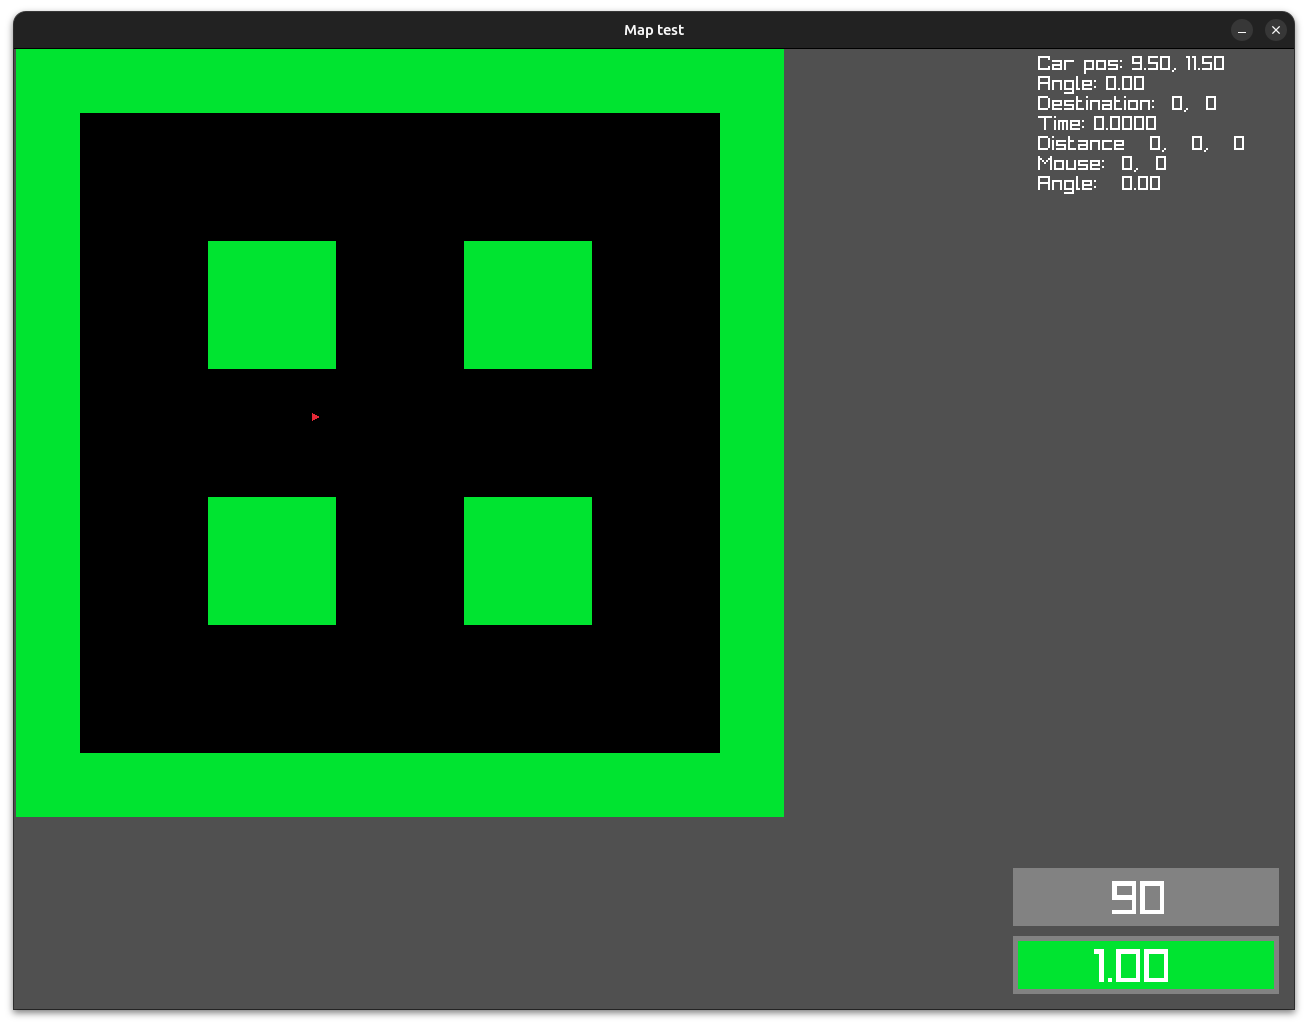
\includegraphics[width = 0.7\textwidth]{PathFinding/App.png}
        \caption{Interfejs aplikacji}
        \label{fig:app}
    \end{figure}
    Interfejs aplikacji składa się z trzech części:
    \begin{enumerate}
        \item Mapa -- reprezentująca aktualnie zbadanego obszar oraz aktualną pozycję pojazdu.
        \item Informacje -- w prawym górnym rogu, wyświetlane są dodatkowe informacje, takie jak aktualna pozycja pojazdu, czy myszy.
        \item Ślizgacze -- w prawym dolnym rogu, znajdują się dwa ślizgacze, górny pozwala precyzyjnie ustawić kąt skrętu kół a dolny pozwala na ustawienie prędkości pojazdu.
    \end{enumerate}

    \subsection{Budowa mapy}
        W założeniu aplikacja ma pozwalać jedynie na wyświetlanie, mapy zbudowanej przez samochód.
        Natomiast wszystkie obliczenia powinny zostać wykonane przez kontroler zarządzający pojazdem.
        Jednak ze względu na duże skomplikowanie opisywanych problemów, w celach testowych, to aplikacja posiada zaimplementowany algorytm do wyszukiwania ścieżek.
        Następnie wyznaczona ścieżka zamieniana jest na proste instrukcje w stylu ,,uruchom oba silniki na 500mm'' czy ,,skręć kołami o $30^\circ$ w lewo''.
        



    \subsection{Wyznaczanie ścieżek}
        Kliknięcie na mapę, pozwala na wybranie punktu docelowego, do które zostanie wyznaczona ścieżka, po której pojazd będzie się poruszał.

        \subsubsection{Algorytm odnajdowania ścieżek}
            Wyznaczanie optymalnej ścieżki, od wielu lat jest bardzo popularnym problemem w informatyce i robotyce.
            Istnieje wiele artykułów, skupiających się na tej tematyce, a także wiele gotowych rozwiązań.
            Najpopularniejszymi algorytmami są:
            \begin{itemize}
                \item algorytm A* (A star),
                \item algorytm Dijkstra,
                \item algorytm Bellmana-Forda.
            \end{itemize}

            Poniżej przedstawione zostaną wyniki pracy \citetitle{AnalizaAlgorytmówŚcieżek} \cite{AnalizaAlgorytmówŚcieżek}
            autorstwa: Beata \citeauthor{AnalizaAlgorytmówŚcieżek}.
            \begin{figure}[!ht]
                \centering
                \figurePlotName
                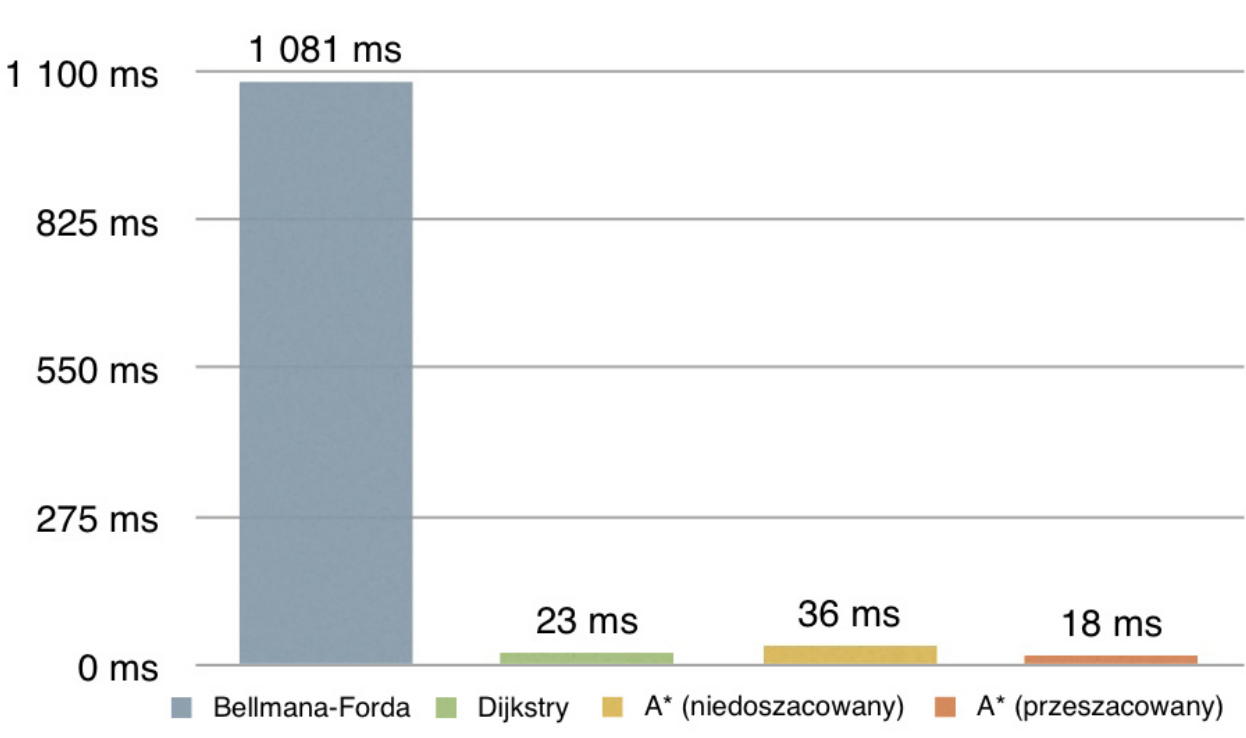
\includegraphics[width=0.7\textwidth]{PathFinding/Wykres_sredni_czas_algorytmu_pathfinding.png}
                \caption{Porównanie średniego czasu wykonania algorytmów}
                Źródło:\cite{AnalizaAlgorytmówŚcieżek} \citetitle{AnalizaAlgorytmówŚcieżek} 
                \label{fig:PathFindingTime}
            \end{figure}
            \begin{figure}[!ht]
                \centering
                \figurePlotName
                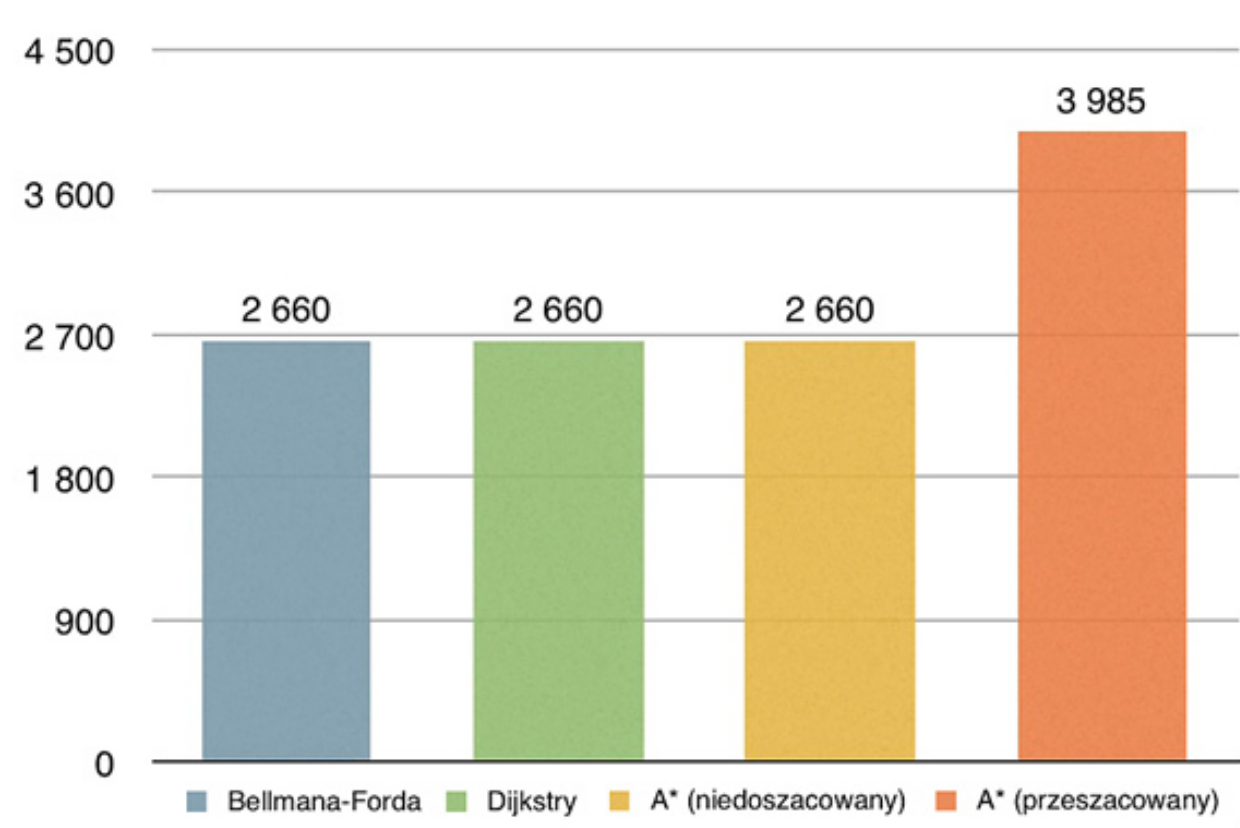
\includegraphics[width=0.7\textwidth]{PathFinding/Wykres_sredni_koszt_algorytmu_pathfinding.png}
                \caption{Porównanie średniego kosztu znalezionych ścieżek}
                Źródło:\cite{AnalizaAlgorytmówŚcieżek} \citetitle{AnalizaAlgorytmówŚcieżek}
                \label{fig:PathFindingCost}
            \end{figure}
            
            Z powyższej pracy wynika, że najlepszym rozwiązaniem jest algorytm Dijkstry.
            Dodatkowym czynnikiem, potwierdzającą powyższe stwierdzenie jest samo skomplikowanie algorytmu.
            Algorytm Dijkstry jest stosunkowo prosty w implementacji, a także posiada niski koszt obliczeniowy.
            Dzięki czemu wydaje się najlepszym rozwiązaniem dla zastosowań w układach embedded.



    
\lsection{Sterowanie pojazdem}
    Sterowanie pojazdem powinno odbywać się w sposób płynny i precyzyjny.
    W poniższym rozdziale zostaną omówione algorytmy, odpowiedzialne za najbardziej podstawowe funkcje poruszania się takie jak: jazda prosto, skręt oraz cofanie.

    \subsection{Jazda przez pewien odcinek}
    \label{subsec:sterowanie_odległość}
        W rozdziale \ref{section:jazda_prosto}, zostały opisane problemy jakie wystąpiły podczas budowy pojazdu. %oraz problemy jakie musiały zostać rozwiązane aby samochód był w stanie jechać prosto.
        Dzięki rozwiązaniu wyżej wymienionych problemów, pojazd był w stanie jechać prosto.
        Jednak dla precyzyjnego sterowania, informacja o tym, że pojazd porusza po linii prostej, jest niewystarczająca.
        Obowiązkowym jest poznanie odległości jaką pokonuje pojazd.

        Wartość odległości jaką pokonuje pojazd od momentu startu, możemy dość dokładnie obliczyć, korzystając ze wzoru \eqref{eq:pulseToDistance}.
        \begin{gather}
            s = \frac{\text{pulse} \cdot 2\pi R}{N}
            \label{eq:pulseToDistance}
        \end{gather}
        gdzie:
        \begin{itemize}
            \item $s$ -- odległość jaką pokonał pojazd,
            \item $\text{pulse}$ -- liczba impulsów z enkodera,
            \item $R$ -- promień koła,
            \item $N$ -- liczba impulsów na obrót koła.
        \end{itemize}

        Wzór ten, można także przekształcić w drugą stronę, aby obliczyć ile impulsów enkodera musi zostać zliczonych, przez procesor aby pojazd pokonał zadaną odległość.
        \begin{gather}
            \text{pulse} = \frac{s \cdot N}{2\pi R}
            \label{eq:distanceToPulse}
        \end{gather}

        Dla zbudowanego modelu, promień koła wynosi $R = 50cm$, a liczba impulsów zgodnie z dokumentacją wynosi $N = 1920$.
        A więc dokładność pomiaru odległości wynosi około:
        \begin{gather}
            \Delta s \approx \pm2.0mm
        \end{gather}


    \subsection{Wyznaczanie zakrętów}
        Wyznaczenie idealnie prostej trasy dla pojazdów nie zawsze jest możliwe.
        W trakcie jazdy, pojazd będzie skręcał wielotonie, w każdym możliwym kierunku.
        Dlatego niezwykle ważne jest, aby zachować maksymalną precyzję podczas skręcania.

        Aby wyznaczyć w jaki sposób nasz samochód powinien skręcić, musi wyznaczyć kilka podstawowych parametrów.
        A są to:
        \begin{itemize}
            \item długość łuku,
            \item promień skrętu,
            \item kąt skrętu kół.
        \end{itemize}
        Na tej podstawie, możemy stworzyć zależność, która pozwoli na napisanie instrukcji dla samochodu, w jaki sposób ma się poruszać.
        \begin{gather}
            s = 2\pi (r(\gamma) + \Delta r) \cdot \frac{\alpha}{360}
            \label{eq:turning_arc}
            \\
            \alpha = \frac{2\pi (r(\gamma + \Delta r))}{s \cdot 360}
        \end{gather}
        gdzie:
        \begin{itemize}
            \item $s$ -- długość łuku,
            \item $r(\gamma)$ -- promień skrętu wyznaczany zgodnie z równaniem \eqref{eq:turning_radius},
            \item $\Delta r$ -- odległość między kołami,
            \item $\alpha$ -- oczekiwany kąt skrętu.
        \end{itemize}

        Dzięki rozważaniom z rozdziału \ref{subsec:sterowanie_odległość}, oraz równaniu \eqref{eq:turning_arc} i \eqref{eq:turning_radius}.
        Możemy stworzyć prostą logikę odpowiedzialną za skręcanie pojazdu.


        \subsubsection{Minimalny promień skrętu}
        \label{subsubsec:minamalny_promien}
            Wyznaczenie promienia skrętu jest 
            \begin{gather}
                2\pi (r + \Delta r) \cdot \frac{\Delta \alpha}{360^\circ} = s\\
                r + \Delta r = \frac{s}{2\pi \cdot \frac{\Delta \alpha}{360^\circ}}
            \end{gather}
            gdzie:
            \begin{itemize}
                \item $r + \Delta r$ -- promień skrętu zewnętrznego koła,
                \item $\Delta \alpha$ -- zakreślony kąt,
                \item $s$ -- długość łuku.
            \end{itemize}

            Zbudowany pojazd, ma możliwość jazdy przez zadaną odległość. 
            Odległość pokonana przez samochód jest dość precyzyjne mierzona przez enkodery,
            a pomiary odległości za pomocą czujników ToF pozwalają na zaufanie dla wartości zadanej.

            Dzięki rozważaniom z rozdziału \ref{subsubsec:dyferencjal} udało się uzyskać powtarzalności pomiarów zakreślonego kąta.
            I tak przykładowo, dla ustawionego maksymalnego kąta skrętu kół $\gamma = 90 \pm 30^\circ$ oraz długości łuku $s = 500mm$, wartość zakreślony kąt wynosił około $\Delta \alpha = \left(60.0 \pm 3.0\right)^\circ$.
            Wartość promienia skrętu wynosiła około:
            \begin{gather}
                r = \frac{500mm}{2\pi \cdot \frac{60 \pm 3.0}{360}} - 125mm \approx (340 \pm 20)mm
            \end{gather}

            Przedstawiony minimalny promień skrętu, możemy oczywiści porównać zgodnie z równaniem \eqref{eq:turning_radius}.
            Po podstawieniu wyżej wymienionych wartości, otrzymujemy:
            \begin{gather}
                r(\gamma = 90 \pm 30^\circ) = \left|\frac{155}{\tan(\pm 30^\circ)}\right| \approx 270mm
            \end{gather}

            Teoretyczny minimalny promień skręty, wychodzący z obliczeń, jest znacząco mniejszy od zmierzonego minimalnego promienia skrętu.
            Wynika to z nie idealności konstrukcji, oraz zastosowania ,,względnie słabej jakości" serwomechanizmu.
            Pojazd nie jest w stanie skręcić kołami jednakowo w obie strony, co wymusiło ustawienie wartości offsetu, przesuwającej wartość kąta skrętu.
            Dla pojazdu testowego, wartość offsetu wynosiła $-6^\circ$. 
            Co ogranicza maksymalny zakres skrętu do $\pm 23^\circ$.
            \begin{gather}
                r(\gamma = 90 \pm 23^\circ) = \left|\frac{155}{\tan(\pm 23^\circ)}\right| \approx 350mm
            \end{gather}


    \section{Podsumowanie}
    Budowa pojazdu autonomicznego, okazała się niełatwym zadaniem.
    Ilość problemów, które występują podczas prac nad takim samochodem okazała olbrzymia.
    Co gorsza napotkane problemy, nie należą do jednej dziedziny.
    Przykładowo, opisany w rozdziale \ref{subsubsec:dyferencjal} problem brakiem dyferencjały, był problemem wynikającym z mechaniki pojazdu, a rozwiązanie pochodzi przyszło od informatycznej strony.

    Z drugiej strony, najbardziej podstawowe algorytmy, będące czysto informatycznymi zagadnieniami, wymagały uwzględnienia mechaniki pojazdu.
    Przykładowo, algorytm wyznaczające trasę w pierwotnej wersji, nie zakładał dzielenia ścieżek na instrukcje a wzorował się na schemacie przedstawionym w pracy \citetitle{Simple_PathSmoothing}\cite{Simple_PathSmoothing}.
    To rozwiązanie po próbie implementacji okazało się nie wystarczające i wymusiło, poszukiwanie innych rozwiązań opisanych w rozdziale \ref{subsec:wygładzanie_ścieżek}.
    Także inne problemy, które wystąpiły podczas budowy, bardzo często pochodziły z jednej dziedziny a jedyne sensowne rozwiązanie pochodziło z drugiej.

    Podsumowując pomimo przedstawionych problemów, udało sie zbudować i odpowiednio oprogramować samochód.
    Aktualny projekt można z pełną odpowiedzialnością nazwać pojazdem antonimicznym.



    \vfill
    \begin{flushright}
        Łukasz Przystupa
    \end{flushright}

    \newpage
    \pagenumbering{gobble}
    \nocite{*}
    \printbibliography

\end{document}
